\documentclass[twoside]{dissertation}
\usepackage{amsthm}
\usepackage{fontspec}
\usepackage{multirow}
\usepackage{stmaryrd}
\usepackage{pifont}
\usepackage{comment}
\usepackage{framed}
\usepackage{rotating}
\usepackage[T1]{fontenc}
\usepackage{srcltx}
\usepackage{enumerate}
\usepackage{relsize}
\usepackage{booktabs}
\usepackage{caption}  
\usepackage{phaistos}

\newtheoremstyle{break}{}{}{\itshape}{}{\bfseries}{.}{\newline}{}

\theoremstyle{definition}
\theoremstyle{break}
\newtheorem{syntax}{Definition}
\newtheorem{definition}{Definition}
\theoremstyle{break}
\newtheorem{convention}{Convention}

\begin{document}
\maketitle
\frontmatter
\chapter*{Abstract}

% -----------------------------------------------------------------------------


\chapter*{Dedication and Acknowledgements}

\makedecl
\makeaidecl
\tableofcontents
\listoffigures
\listoftables

% -----------------------------------------------------------------------------

\chapter*{Ethics Statement}

% -----------------------------------------------------------------------------

\chapter*{Supporting Technologies}
\label{chap:supporting_tech}

\begin{quote}
\noindent
\begin{itemize}
\item I used React (\url{https://react.dev/}) to develop the website for this project.
\item The bindings for the web assembly interface to the library for the language were generated by using macros from the wasm-pack rust crate: \url{https://github.com/rustwasm/wasm-pack}.
\item I used GitHub Copilot to help assist with generating unit tests.
\end{itemize}
\end{quote}

% -----------------------------------------------------------------------------

\chapter*{Notation and Acronyms}
\begin{acronym}
\acro{SFL}{Simple Functional Language}
\acro{FP}{Functional Programming}
\acro{WASM}{Web ASseMbly}
\acro{CLI}{Command Line Interface}
\end{acronym}
\mainmatter
\chapter{Introduction}
\label{chap:context}

In this dissertation I present SFL-explorer: a tool to demonstrate how functional programming languages are evaluated, allowing users to gain a valuable intuition of these languages.

SFL-explorer takes the form of a functional language (\ac{SFL}), packaged with two interfaces that allows users to observe the process of evaluation of a term as a series of step by step or multi-step reductions, and control the order that sub-terms are evaluated. These interfaces are a \ac{CLI} and a web application. The ultimate goal of this project was to make a tool that makes learning and teaching the basics of functional programming easier. There are two groups of people the project is designed to be of interest to:
\begin{itemize}
    \item Those involved in learning functional languages. These could be students of a university course, or anyone interested in the topic. 
    \item Those involved in teaching functional languages, as part of a university course or otherwise.
\end{itemize}

The language itself is not meant to be the main interest for the users of this system. It is designed to be fairly generic, with syntax and semantics similar to popular functional languages, so that users can take their understanding from using SFL-explorer and apply it to these languages. 


\chapter{Background}
\label{chap:technical}

\section{The Lambda Calculus}
\label{bg:lcalc}
\newcommand{\lcalc}{$\lambda$-calculus}
\newcommand{\lCalc}{$\lambda$-Calculus}
\newcommand{\fto}{\rightarrow}
The lambda calculus (\lcalc) was first described by Alonzo Church in 1936~\cite{church1936unsolvable}. It is a universal model of computation, meaning we can compute any computable function using it~\cite{Turing_1937}. Understanding the \lcalc\ is essential for understanding the principles behind functional languages and in particular how they evaluate expressions.

The set of all lambda terms is $\Lambda$. Lambda calculus is built from three syntax structures:
\begin{itemize}
    \item Variables, selected from an infinite set of variables $V=\{x,y,z,\dots\}$
    \item Abstractions, $\lambda x. M$ which are functions, where we `bind' a variable $x$ for use in the term $M$ such that when we apply our function to a term $N$, all instances of $x$ in $M$ are substituted with $N$.
    \item Applications $M N$ where we apply a term $M$ to an argument $N$. 
\end{itemize}

\noindent Below is a more formal definition of the \lcalc~\cite{barendregt2013lambda}.
\begin{alignat*}{3}
&x \in V                 \quad && \implies \quad && x \in \Lambda               \\
&M,N \in \Lambda         \quad && \implies \quad && (M N) \in \Lambda           \\
&M \in \Lambda, x\in V   \quad && \implies \quad && (\lambda x. M) \in \Lambda  
\end{alignat*}

\noindent We shall also use the following fairly standard conventions:

\begin{enumerate}
    \item Application is left associative. The term $M_1\,M_2\,M_3$ means $(M_1\,M_2)\,M_3$ and not $M_1\,(M_2\,M_3)$
    \item Nested abstractions can be grouped: the term $\lambda x \;y. M$ means $(\lambda x . (\lambda\;y. \;M))$.
    \item Outermost parenthesis are omitted.
    \item The body of an abstraction extends as far to the right as possible: the term $\lambda x. M\,N$ means $(\lambda x. (M\;N))$ and not $((\lambda x. M)\,N)$. 
\end{enumerate}

\subsection{Free variables}
\begin{quotation}
\noindent`An occurrence of $x$ is free if it appears in a position where it is not bound by an enclosing abstraction on $x$' \cite{pierce2002types}
\end{quotation}

\noindent Free variables are a useful concept to express which variables are `ready for substitution' in a term. Formally, the function $FV(M)$ is the set of free variables in the term $M$ \cite{barendregt2013lambda}:
\begin{alignat*}{3}
FV(x)              \quad && = \quad && &\{x\}               \\
FV(M\,N)           \quad && = \quad && &FV(M)\union FV(N)   \\
FV(\lambda x. M)   \quad && = \quad && &FV(M)-\{x\}         \\
\end{alignat*}

\noindent A term is \textit{closed} if it has no free variables, and \textit{open} if it does. 

\subsection{Reduction}
\begin{quotation}
\noindent`The sole means by which terms `compute' is the application of functions to arguments (which themselves are functions). Each step in the computation consists of rewriting an application whose left-hand component is an abstraction, by substituting the right-hand component for the bound variable in the abstraction's body' \cite{pierce2002types} 
\end{quotation}

\noindent The \lcalc\ is evaluated by $\beta$-reduction. This is where an abstraction is applied to a value. The result of applying an abstraction to a term is the body of the abstraction, with the all free instances of the abstracted variable substituted with the term the abstraction was applied to. Below is the formal definition of substitution within a term~\cite{barendregt2013lambda}. 
\noindent\begin{alignat*}{3}
&x[x:=N]                        \quad && \equiv \quad && N                       \\
&y[x:=N] \text{ where } y \ne x \quad && \equiv \quad && y                       \\
&(M_1 M_2)[x:=N]                \quad && \equiv \quad && (M_1[x:=N]) (M_2[x:=N]) \\
&(\lambda y.M)[x:=N]            \quad && \equiv \quad && \lambda y.(M[x:=N])     
\end{alignat*}  
\noindent The definition of $\beta$-reduction \cite{barendregt2013lambda}:
\begin{alignat*}{3}
&x                 \quad && \BetaReduce \quad &&        x           \\
&\lambda x.M       \quad && \BetaReduce \quad &&        \lambda x.M \\
&(\lambda x.M) N   \quad && \BetaReduce \quad &&        M[x:=N]
\end{alignat*}
A term is said to be in \textbf{normal form} if it cannot be $\beta$-reduced. A term that can be beta reduced can be said to be a \textbf{redex}: a reducible expression. The term resulting from the redex is a \textbf{contraction}.

\subsection{Reduction, Evaluation Strategies and Values}
\label{bg:eval_strategies}
We often have a term where we have multiple options for $\beta$-reduction. In this section, we will briefly discuss three different evaluation strategies that inform which option is selected during evaluation: call-by-value (a.k.a. strict), call-by-name and call-by-need (a.k.a. lazy). When a term is fully reduced under a given evaluation strategy, we say that it is a value. Below is an example of each evaluation strategy. I have used the same examples as Pierce~\cite{pierce2002types}. 

The closed term 
\((\lam{x} x)\,((\lam{x} x)\,(\lam{z} (\lam{x}. x) z))\) has three redexes ($id$ is shorthand for $\lam{x} x$):
\[\underline{id\,(id\,(\lam{z} id\,z))}\]
\[id\,\underline{(id\,(\lam{z} id\,z))}\]
\[id\,(id\,(\lam{z} \underline{id\,z}))\]

\noindent Most languages use the \textbf{call-by-value} evaluation strategy, where `only the outermost redexes are reduced and a redex is reduced only when its right-hand side has already been reduced to a value \ldots\ where the only values are \lambda expressions'~\cite{pierce2002types}. This reduction strategy is also known as `strict'. In this strategy, we would reduce by the following sequence:
\begin{alignat*}{2}
id\,\underline{(id\,(\lam{z} id z))}  && \;\;\arr\\ 
(\underline{id\,(\lam{z} id z)})      && \;\;\arr\\ 
(\lam{z} id z)                        && \;\;\\ 
\end{alignat*}

\noindent Using the \textbf{call-by-name} strategy, `The leftmost outermost redex is always reduced first \ldots\ and [we allow] no reductions inside abstractions' \cite{pierce2002types}. Only abstractions are valid values. Our reduction sequence would look like this:
\begin{alignat*}{2}
\underline{id\,(id\,(\lam{z} id z))}  && \;\;\arr\\ 
(\underline{id\,(\lam{z} id z)})      && \;\;\arr\\ 
(\lam{z} id z)                        && \;\;\\ 
\end{alignat*}
\noindent \textbf{Call-by-need} is similar to call by name but with sharing. This means we `overwrite all occurrences of an argument with the value the first time it is evaluated' \cite{pierce2002types}. Only abstractions are valid values once again. This is an optimization of call-by-name that is known as lazy evaluation. It is used by many functional languages including Haskell, and is of particular importance to SFL explorer. In this case, our reduction order would be the same as \textbf{call-by-name}. 

% \sam{these are all standard, so you should cite where they come from and explain them. Spend more time on reduction, because that will be key later}
% \sam{this section is very dry. why do we want to learn about lambda calc? well we are writing an evaluator, so to understand what that means we need to understand syntax and evaluation, so lets looks at the lambda calc as a small example. It makes the intro of lambda calc more active and motivated, rather than a bunch of dry definitions, instead its a small example of what we will do later, that is background cos its pre-defined and not implemented we are just exploring the ideas we will implement}

\subsection{Types}
If we were to extend our \lcalc\ with a new sort of term, an integer literal (something commonly done, especially when building up to discussing practical functional languages) \[\dots, -2, -1, 0, 1, 2, \dots\] we could say that these values are members of a set of values $Int$. 

In this extended version of the lambda calculus, the set of valid values becomes:
\[Values ::= \lambda x. M \mid \dots \mid -2\mid -1\mid 0\mid 1\mid 2\mid \dots \]

\noindent It would be useful for us to be able to assert that a term eventually evaluates to one of these $Int$s. The \lcalc\ terms that evaluate to a value in the set of $Int$s can all be said to have `type' $Int$. More generally: 
\begin{quote}
`Saying that `a term $t$ has type $T$' (or `$t$ belongs to $T$' or `$t$ is an element of $T$') means that $t$ `obviously' evaluates to a value of the appropriate form - where by `obviously' we mean that we can see this statically, without doing any evaluation of $t$' \cite{pierce2002types}
\end{quote}

\noindent For instance, the term \((\lam{x} 1)\, 2\) has type $Int$, as it evaluates to a value in the set of valid $Int$ values. 

% \sam{i havent read further of lambda calc, cos i think my above advise applies here too. 1. you are burdened with too much knowledge so you keep jumping into the middle of an explanation 2. it is unclear why we are learning about types 3. remember lambda calc is a whole 3rd year course, and you've seen how long stevens notes are, we cannot replicate that so we need to highlight to the user what is important to understand about the lambda calc for just this project}

\subsubsection{Functions}
We want to be able to express the types of functions. The term \(\lambda x. x\) can be said to have type \(T \fto T\), as it takes in a term of type $T$ and returns the same term, which still has type $T$.

A more complex term \(\lambda x\;y.x\) can be said to have type \(T \fto (U \fto T)\); If we give it a term $M$ of type $T$, it would return the function \(\lambda y.M\) which takes whatever is given to it (represented by $U$) and returns $M$ which has type $T$. 

% \subsubsection{Judgements}
% \todo{To make typechecking bit easier}

% By convention, $\fto$ is right associative so way may omit the right most parenthesis. 

\subsection{Typechecking: Well typed programs do not go wrong}
The \lcalc\ that we have discussed so far is untyped. This means that an abstraction can be applied to any other term without restriction. This lack of restriction may result in terms that can no longer be reduced, but are not valid values. The evaluation of an \lcalc\ expression is said to have `gone wrong' if it gets to a normal form that is not a valid value.

Let us consider the expression and its reduction
\[
(\lambda x. x\;x) \;1 \BetaReduce 1\;1
\]
\noindent The reduction is not a valid value, however it cannot be further reduced. We have \textit{gone wrong}.

We will now attempt to derive the type of the parameter $x$, in order to show that it is untypeable.
As $x$ here is applied to itself, it must be some kind of function that takes a term $x$ of with type $T$, and returns a term of type $U$. This means that $T = T \fto U$ which is absurd, as it is left recursive. This means that this is `untypeable'. Indeed, it is clearly never possible to type an expression where a term is applied to itself. If this was a real programming language, when it got to the normal form \(1\;1\), we would have to have some form of runtime error. In this case, only permitting typeable terms would have prevented us from \textit{going wrong}, as this term would not have been permitted. 

In general, \textbf{well typed programs do not go wrong} \cite{MILNER1978348}. Therefore, if we are able to exclude all terms in our functional language that are untypeable, we will be able to guarantee that it does not go wrong, and thus prevent these runtime errors. The system that looks at a program statically to decide whether it is well typed is called the \textbf{typechecker}. Types can often also be derived without them needing to be manually specified. This is called \textbf{type inference}.

\section{Haskell: A Functional Programming Language}
Functional programming languages are programming languages where `computation is carried out entirely through the evaluation of expressions' \cite{hudak1989conceptionfunctionalprogranning}. Functional programming languages are based on the lambda calculus. In this section, we will discuss a prolific example of a functional langauge: Haskell. 

Haskell is a very prominent functional programming language that is widely taught. It is a programming language specifically designed to be suitable for teaching \cite{hudak2007history}. This dissertation involves the development of a programming language with some similar features to Haskell, so the corresponding Haskell features and ideas will be introduced here. 

\subsection{Declarations}
Haskell, along with most other languages, provides the facility to name functions and other terms for reference elsewhere in the program. These can be typed, but the types can almost always be inferred. 

Some examples of these declarations, all typed for clarity, are below. For instance, the top level declaration
\begin{lstlisting}[language=SFL]
x :: Int
x = 5
\end{lstlisting}
means that $x$ is equal to $5$. We can also name lambda functions:
\begin{lstlisting}[language=SFL]
add :: Int -> Int -> Int
add = \x y -> x + y
\end{lstlisting}
This can also be written as:
\begin{lstlisting}[language=SFL]
add :: Int -> Int -> Int
add x y = x + y
\end{lstlisting}
\subsection{Polymorphic functions}
In Haskell, functions can be written that operate on values of various types. 

\begin{lstlisting}[language=SFL]
id :: a -> a
id x = x
\end{lstlisting}
\noindent Here, we define the function \sflinline{id} which simply returns its argument. `a' in the type signature represents any type, and can be substituted for any type. The two `a's in the type signature must represent the same type however, mandating that the argument to \sflinline{id} and its return value must be the same type.  

\subsection{User Defined Algebraic Data Types}
\label{bg:haskell_udt}
Many languages, including Haskell, have Algebraic Data Types allowing us to `Compose' other data types. The set of all values of an algebraic data type is isomorphic to an expression involving the sets of values of their constituent types, combined using `set algebra' operations. Haskell allows for `union' and `product' types.  

Haskell allows users to define their own algebraic data types using the \lstinline[language=SFL]|data| keyword. For instance, booleans can be defined:

\begin{lstlisting}[language=SFL]
data Bool = True | False
\end{lstlisting} 

\noindent This data definition creates a type $Bool$ with two data constructors, \verb|True| and \verb|False|. These data constructors are zero-ary. We can also have data constructors that have arguments. 

An example of a union type in Haskell is the tagged union:
\begin{lstlisting}[language=SFL]
data Shape = Circle Int | Rectangle Int Int
\end{lstlisting} 
\noindent which is isomorphic to the type \(Int \cup (Int \times Int)\). 

An example of a product type is the tuple \((Int, Bool)\): the set of all possible values of this type is isomorphic to the Cartesian product of the set of all values of \(Int\) and the set of all values of $Bool$. Most languages have product types, which often take the form of structs or tuples. 

\subsection{Polymorphic Type Constructors}
Haskell includes polymorphic types. These are `types that are universally quantified in some way over all types'~\cite{hudak1992gentle}. One example is the type constructor $Maybe$, implicitly created by the following data declaration.

\begin{lstlisting}[language=SFL]
data Maybe a = Just a | Nothing
\end{lstlisting} 

This creates a \textit{type constructor} called \(Maybe\), as well as $Just$ and $Nothing$ which are data constructors. $Maybe$ represents a constructor that takes a type, and returns a concrete type (a type that is not a type constructor). Type constructors are also types. This is first-order polymorphism, as opposed to higher-order polymorphism where a type can be an `abstraction over type constructors'. \cite{yallop2014lightweightpoly}. 

The `Type of a Type' is its \emph{kind} \cite{pierce2002types}. For example, the type constructor $Maybe$ has the kind $* \fto *$. This notation looks similar to how functions over values are defined, reflecting the fact that $Maybe$ behaves like a function, but at the type level rather than the value level. If we were to apply the constructor \(Maybe\) to the concrete type \(Int\), the resulting type would be the concrete type \(Maybe \;Int\). 

\begin{lstlisting}[language=SFL]
data Either a b = Left a | Right b
\end{lstlisting} 

Here, $Either$ is a type constructor with the kind $* \fto * \fto *$, meaning it takes two concrete types and returns a concrete type. 

\subsection{Pattern Matching}
\label{bg:haskell_pattern_match}
Haskell allows us to do pattern matching, allowing conditional execution based on whether a term matches a given form. The following function would have different results depending on whether the input value was 0 or another integer.

\begin{lstlisting}[language=SFL]
isZero :: Int -> Bool
isZero 0 = true
isZero _ = false
\end{lstlisting}

\noindent The underscore `\verb|_|' represents a wildcard pattern that matches anything. In this case, it matches any $Int$ that is not $0$. We can match more complicated expressions, and assign variables throughout the pattern.

\begin{lstlisting}[language=SFL]
data SomeValues a = One a | Two a a | Three a a a | Four a a a a

valuesToList :: SomeValues a -> [a]
valuesToList (One x) = [x]
valuesToList (Two x1 x2) = [x1, x2]
valuesToList (Three x1 x2 x3) = [x1, x2, x3]
valuesToList (Four x1 x2 x3 x4) = [x1, x2, x3, x4]
\end{lstlisting}

\noindent In the first match case of \verb|valuesToList|, we assign the variable $x$ to be the term of type $a$ that the data constructor \sflinline{One} is applied to. In the second, we assign \verb|x1| and \verb|x2| to be the first and second term of type $a$ that the constructor \sflinline{Two} is applied to etc. 

\section{Rust}
\label{bg:rust}

This project is written in rust, to take advantage of rusts unique mix of speed, and high level language features. Some of the decisions made, particularly in the implementation of the AST, require an understanding of Rust, especially the memory management model.

`Ownership' is an important concept. The rules of ownership \cite{rust_book}:
\begin{itemize}
    \item Each value in Rust has an owner.
    \item There can only be one owner at a time.
    \item When the owner goes out of scope, the value will be dropped.
\end{itemize}   

If a value is owned in one scope, but another scope needs to read/write it, we may use a reference to the value. The rules of references \cite{rust_book}:
\begin{itemize}
    \item At any given time, you can have either one mutable reference or any number of immutable references. 
    \item References must always be valid.
\end{itemize}

These rules ensure that immutable references are to things that don't change, and all references are always to things that exist.

\section{Frontend Technologies}
\label{bg:frontend}
\label{bg:pwa}
\begin{itemize}
    \item Vite
    \item React
    \item NPM
    \item PWAs
\end{itemize}


\section{Web Assembly} \label{bg:wasm}
This project runs entirely within the browser, despite being written in Rust. This is due to the fact that it compiles to web assembly. Automated tools exist for the generation of JavaScript bindings around Rust functions/types, but this process places certain restrictions around functions arguments and return types. 

We will discuss this here to allow us to refer to these restrictions, and also to explain the process of compiling and using Rust code in a modern web browser. 

Web Assembly 2.0 is a 32 bit target~\cite{WebAssemblyCoreSpecification2}. This means we only have 4GB of addressable memory. The Rust compiler is based on LLVM, which provides a web-assembly compilation target. The Rust compiler has a toolchain around this compilation target, that allows for easy compilation to web-assembly. However, this only creates a binary blob, which requires more work to make interoperable with our JavaScript build system (Vite). We must do two things to achieve interoperability:
\begin{itemize}
    \item Incorporate it into our build so it can be served with it.
    \item Load the WASM package in a way that allows for us to call the functions.
\end{itemize}
Producing an NPM package with some JavaScript functions that call the WebAssembly functions would achieve both of these goals. However, if we wish to use TypeScript, we must create a separate type definition file that contains the types of all of the JavaScript wrapper functions around the WASM functions. This would be difficult to maintain manually as we would have to update it every time we made a change to the public interface of our rust library. 

Fortunately, the rust crate \verb|wasm-bindgen| provides macros that generate a whole NPM package, including TS bindings, automatically. This package can then be added as a dependency to an NPM app that provides a website, and the functions within it can [TODO: WASM-bindgen vs WASM pack?]

\paragraph{wasm-pack}
\label{bg:wasm-pack}

\section{Existing systems}
Below are the most relevant existing systems for SFL explorer. 
% https://dl.acm.org/doi/pdf/10.1145/1480828.1480845
% lit review  in previous diss: https://research.ou.nl/ws/portalfiles/portal/31271878/Nicasi_K_IM9906_AF_SE_scriptie_PURE.pdf
% \subsection{WinHIPE}
% https://dl.acm.org/doi/pdf/10.1145/1273039.1273042

\subsection{Duet, and Duet Delta}
\label{bg:duet}
Duet is:

\begin{quotation}
`A tiny language, a subset of Haskell (with type classes) aimed at aiding teachers to teach Haskell'~\cite{duet_hackage}
\end{quotation}

\begin{figure}[h]
    \centering
    \begin{tabular}{c}
    \hline
    \begin{lstlisting}[language=SFL_noprelude_numbers]
data List a = Nil | Cons a (List a)
foldr = \f z l ->
  case l of
    Nil -> z
    Cons x xs -> f x (foldr f z xs)
foldl = \f z l ->
  case l of
    Nil -> z
    Cons x xs -> foldl f (f z x) xs
list = (Cons True (Cons False Nil))

main = foldr _f _nil list
\end{lstlisting}\\ \hline

    \end{tabular}
    \caption{An example Duet program provided in the repository. \_f and \_nil are not defined, but the underscore indicates that this is fine and they should just be left unchanged}
    \label{bg:duet_foldr}
\end{figure}

\begin{figure}[h]
    \centering
    \begin{tabular}{c}
    \hline
    \begin{lstlisting}[language=SFL_noprelude_numbers]
foldr _f _nil list
(\f z l ->
    case l of
        Nil -> z
        Cons x xs -> f x (foldr f z xs))
    _f
    _nil
    list
(\z l ->
    case l of
        Nil -> z
        Cons x xs -> _f x (foldr _f z xs))
    _nil
    list

... 

_f True
  (_f False
     ((\l ->
         case l of
           Nil -> _nil
           Cons x xs -> _f x (foldr _f _nil xs))
        Nil))
_f True
  (_f False
     (case Nil of
        Nil -> _nil
        Cons x xs -> _f x (foldr _f _nil xs)))
_f True (_f False _nil)
\end{lstlisting}\\ \hline

    \end{tabular}
    \caption{The output of evaluating the program shown in Figure \ref{bg:duet_foldr}. The beginning and end are shown, with the middle removed. }
    \label{bg:duet_foldr_eval}
\end{figure}

\noindent When running Duet \cite{duet_hackage} on the program shown \ref{bg:duet_foldr}, we get a large block of text as output that shows the reduction or this program. This all happens at once, and we do not get the chance to pick reduction order. It is also quite hard to tell what is going on, as it is dumped as one block of text. The author, Chris Done, also hosts a website where one can try it out without installing it c \cite{duet_delta}. The website does not provide much in the way of a UI, it is a text box input and a text box output for running Duet programs.

\noindent The main strong point of this project is the language. It is a solid subset of Haskell that includes many similar features to SFL. For this project, I did not draw direct inspiration from Duet or Duet Delta. This was because even though I liked the subset of Haskell selected for Duet, I wanted to attempt to design a clearer language, and potentially break away from being a Haskell subset. Furthermore, Duet and Duet Delta focus on the language, not the UX/UI, whereas I wanted SFL explorer to be strong in both regards. 

\subsection{$\lambda$-Lessons}
\newcommand{\llessons}{$\lambda$-Lessons}
\label{bg:llessons}

\llessons\ is a website created by Jan Paul Posma and Steve Krouse at YC Hacks '14 \cite{lambdalessons}. It is a very effective demonstration of `map', `foldr' and `foldl:

\begin{quotation}
\noindent It is `A short, interactive lesson that teaches core functional programming concepts. It was designed to transform the way you think about performing operations on lists of things, by showing you how functions are executed' \cite{lambdalessons}
\end{quotation}

\noindent It is unfortunate I only found out about it at the end of phase 4 of the project, otherwise my project could have drawn inspiration in terms of UI for free choice evaluation. Indeed, I only discovered this project through correspondence with Chris Done, the author of Duet \ref{bg:duet}. Despite the fact that my project did not take inspiration from this system, it would be remiss not to mention it. 

My particular favorite features of \llessons's UI are:

\begin{itemize}
    \item It allows the user to select in the code what part they want to reduce next by clicking on it. 
    \item It shows informations about functions when you hover over them in the source code. 
\end{itemize}


\begin{figure}[t]
    \centering
    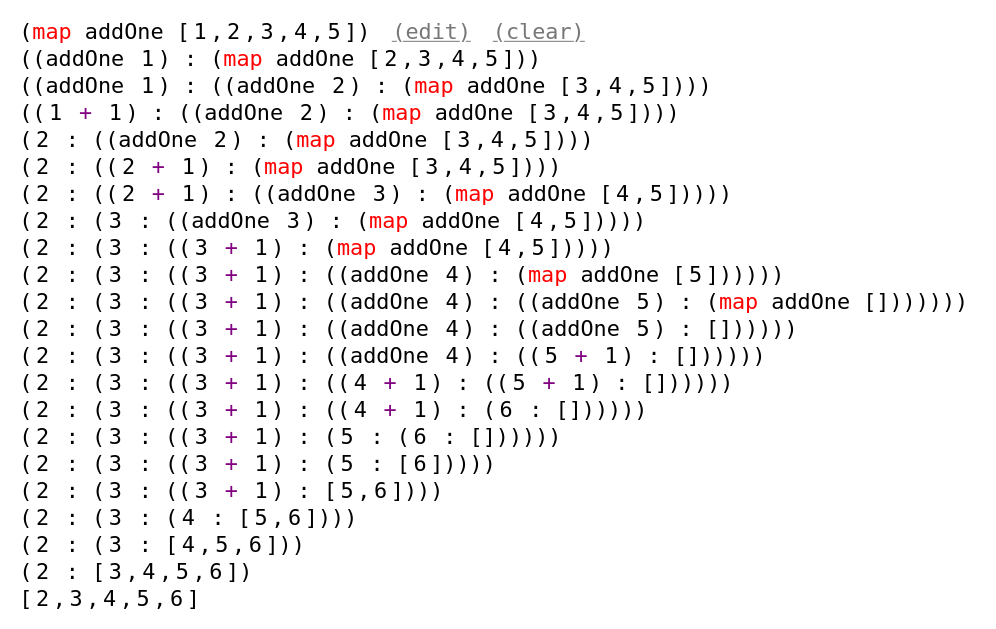
\includegraphics[width=0.75\linewidth]{images/LLessonsMap.png}
    \caption{Evaluation of\ `\sflinline{map addOne [1, 2, 3, 4, 5]}'\ with \llessons}
    \label{bg:llessons_ui}
\end{figure}

\begin{figure}[t]
    \centering
    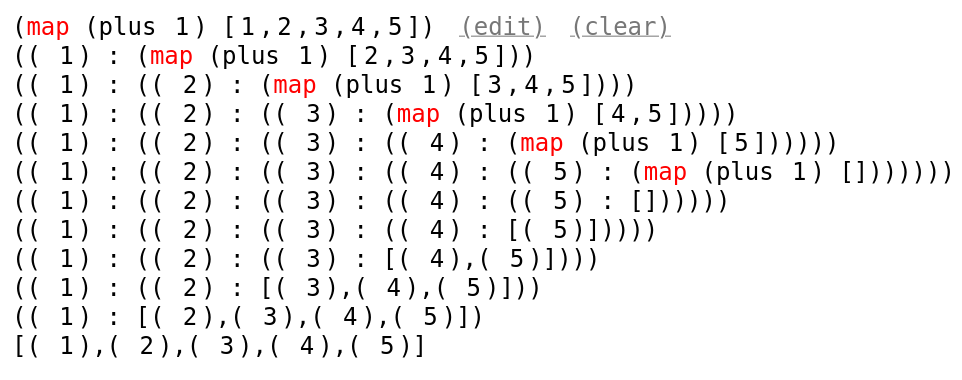
\includegraphics[width=0.75\linewidth]{images/LLessonsGoingWrong.png}
    \caption{Evaluation of `\sflinline{map (plus 1) [1, 2, 3, 4, 5]}' with \llessons. It gets confused by currying and partial application}
    \label{bg:llessons_gets_confused}
\end{figure}

The UX/UI is the definite strong point of \llessons\ (see \ref{bg:llessons_ui}).  However, there are a few things that I would identify as weaknesses that make it not useful for what SFL explorer is useful for.

\begin{itemize}
    \item The language is not typechecked. There are type assignments, but upon testing and inspection of the source code \cite{lambdalessonsgithub}, type assignments are ignored. They say on the website that the language is `dynamically typed'~\cite{lambdalessons}, but it is not. 
    \item The language does not allow for user defined algebraic data types, but it has \sflinline{List} built in. 
    \item As can be seen in \ref{bg:llessons_ui}, it seems to imply that \sflinline{((x : y : []))} reduces to \sflinline{[x, y]} which is misleading, as these two are infact identical. 
    \item The language does not support lambda functions.
    \item The language does not support currying or partially applying functions (\ref{bg:llessons_gets_confused}).
    \item The program states are not saved between refreshes. 
\end{itemize} 

\noindent In summary, \llessons\ is designed for a different purpose than SFL Explorer. It describes itself as a `document'~\cite{lambdalessons} rather than an all around teaching tool for functional languages. It does not provide much capability to experiment yourself outside of `map' and `fold' as the language is not very extensive. However, the ability to reduce an expression by clicking on the section of the expression you want to reduce is very intuitive, and inspiration could definitely be drawn from this for any future iterations of SFL Explorer. 

% \subsection{Other Notable Mentions}
% Unfortunately, I do not have the page count to spare to go into detail about some of the other existing systems identified. Here are some of my favorites, along with a brief summary of their achievements. 

% \begin{itemize}
%     \item WinHIPE \cite{WinHIPE}
% \end{itemize}

% \subsection{Conclusion of Research on Existing Systems}


% https://stevekrouse.github.io/hs.js/

\section{COMS10016: Imperative and Functional Programming at the University of Bristol}
\label{COMS10016}
In the first year of most computer science programs at the University of Bristol, students take the module \href{https://www.bristol.ac.uk/unit-programme-catalogue/UnitDetails.jsa?unitCode=COMS10016}{COMS10016}, a combined imperative and functional programming module. This is many students first encounter with both of these types of programming. In the functional part of this unit, students are taught Haskell. The unit material is presented to students through a series of lectures, supplemented by weekly worksheets that students have the opportunity to work through in labs attended by the lecturers, as well as some teaching assistants. Two of the lecturers in this unit are Jess Foster and Samantha Frohlich. 

\begin{quote}
`The aim [of the functional portion of the unit] is to introduce types and functions. Important principles include datatypes, evaluation order, higher-order functions, and purity' \cite{COMS10016}
\end{quote}

\noindent I acted as a teaching assistant in the labs for two academic years. My role was to answer students questions about functional languages or the worksheets they were given. The inspiration for this project came from my experience struggling to explain key functional programming concepts. I frequently needed to resort to writing out the evaluation sequence for a term.
\chapter{Design}
\label{chap:design}

\section{Language Design}
\subsection{Goals}
\label{design:goals}
SFL is designed with the following goals in mind:
\begin{enumerate}
    \item SFL should be similar to existing functional languages.
    \item SFL should be simple and easy to understand. 
    \item SFL should be powerful.
\end{enumerate}
The features that should be selected for SFL are the features that maximise these goals for the minimum implementation complexity. The language's syntax and type system should also work towards these goals. 

Out of our design goals, 2 and 3 have the potential to be in conflict, as more expressive power often requires more complex syntax. We must ensure a sensible compromise between all of our goals, while accounting for implementation complexity. 

When adding features for the language, we must prioritise the "core" features of functional languages, and de-prioritise features that are not so "core" to the understanding of functional languages. 

yadadada we should implement features that allow us to implement
\begin{itemize}
    \item Complex data structures, lists and trees
    \item Fold
    \item IO???
\end{itemize}

\subsection{Definitions}

\begin{syntax}[Lowercase and Uppercase ID syntax as regular expressions]
\label{def:identifier_syntax}
(Lowercase Identifier): \(id ::= [a..z][a..zA..Z0..9\_]*\)\newline
(Uppercase Identifier): \(Id ::= [A..Z][a..zA..Z0..9\_]*\)
\end{syntax}

\subsection{Basic Syntax}
Lambda calculus is the basis of modern functional programming languages. As discussed in the background, Lambda calculus consists of 3 structures: identifiers, application, and abstraction. One common extra structure that functional languages implement is an assignment. This is where we label an identifier with a certain meaning, such that all references to the assignment henceforth are identical to a reference to the meaning assigned. For instance:
\begin{lstlisting}[]
f = (\x.x)
main = f y
\end{lstlisting}
Is identical to
\begin{lstlisting}[]
main = (\x.x) y
\end{lstlisting}
Note the use of \verb|"\"| instead of \(\lambda\) as it is the closest character available on most keyboards. A program is then defined as a set of assignments, and we pick one specific label name to mark the "entry-point" expression in the program. Haskell, as well as many other languages, use "main" to represent a programs entry point, so we may use main. 

We must also add a way to represent values, such as integers and booleans, to our language. Most programming languages, including functional ones, at least support integers. Booleans are also often supported to represent the results of integer comparison. Without literal values, programs would have to use complicated encodings (such as church numerals) to represent these values, making programs look more complicated. 

These two features massively shorten and simplify programming in this language.

\begin{syntax}[The basic syntax of SFL]
(Expression) \(E ::= [-][0, 1, ..] \mid true \mid false \mid id \mid \setminus id. E \mid E\:F\)\newline
(Assignment) \(A ::= id = E\)\newline
(Module) \(M ::= A\: M \mid End\)
\end{syntax}

\subsection{Type System}
We must have types representing integers and booleans in our language, if we are to effectively check the validity of expression containing their respective literals. 

Many languages, including Haskell, also have Algebraic Data Types allowing us to "Compose" other data types. Algebraic data types are isomorphic to an algebraic expression consisting of sums and products of their constituent types. An example of a product type is the tuple \((Int,Bool)\) which is isomorphic to \(Int \times Bool\). Most languages have product types, which often take the form of structs or tuples. 
An example of a sum type is the Haskell syntax tagged union:

\noindent\verb!"data Shape = Circle Int | Rectangle Int Int"!, which is isomorphic to the type \(Int + (Int \times Int)\). 

We will now consider generic data structures, such as a lists that can hold any value of type $a$, written as \(List\;a\)". Here, \(List\) is not a type in itself, but it represents a constructor that takes a type, and returns a concrete type. We could write this as "$Type \rightarrow Type$", indicating that it behaves like a function, but at the type level rather than the value level. If we were to apply the constructor \(List\) to the concrete type \(Int\), the resulting type would be \(List \;Int\). 

Polymorphism as described here is first order polymorphism, as opposed to higher-order polymorphism (also known as higher-kinded polymorphism) where a type can abstract over a type that abstracts over a type \cite{pierce2002types}. An example of a function that is higher-order polymorphic is a function that takes a function, and then applies it to two differently typed values:
\begin{lstlisting}
applyToBoth f x y = (f x, f y)
\end{lstlisting}
If \verb|f| is to be applied to any type, it must have a type \(\forall a. a\rightarrow a\). This means the type of the function \verb|applyToBoth| must be \(\forall a \;b.(\forall c \rightarrow c) \rightarrow a \rightarrow b \rightarrow (a, b)\)

This requires the ability to parse expressions with nested \verb|foralls|, as well as support during type inference for higher-kinded types. We do not think that this is a priority for the system, as 
These first-order polymorphic type constructors would be useful to have in SFL, with one example of their utility being defining the polymorphic function "\verb|length :: List a -> Int|" which should work regardless of what type the list is over. Higher order polymorphism is less important
The "Type of a Type" is known as its \emph{kind} \cite{pierce2002types}. Another example is the type representing "Either left or right: \(Either \;a\;b\)", that can be defined with its constructors as \verb!data Either a b = Left a | Right b!. "Either" is a type constructor with the kind "Type -> Type -> Type", meaning it takes two concrete types and returns a concrete type. 
Higher-kinded types are types where there are parenthesis in a kind expression, not including the implicit ones implying right associativity: 
"\verb|Type -> Type -> Type|" is implicitly "\verb|Type -> (Type -> Type)|"
We can avoid thinking about kinds by enforcing that a type constructor is always given the correct number of arguments

Supporting tagged unions and tuples in the SFL type system would massively increase the ease of writing complex programs. It would also allow for complex data structures such as trees and lists. 
Type names, as well as constructor names, start with uppercase letters in Haskell. This allows them to be easily differentiated from type variables, as well as regular variables. 
In the below definition of the SFL type system, we define \(\Alpha\) as the set of valid type names starting with uppercase letters defined by \(Id\), and \(\alpha\) as the set of valid type variable names defined by \(id\). 

\begin{syntax}[Types in SFL]
(Inbuilts): \(B::=Int\mid Bool\)\newline
(Monotype): \(\tau, \sigma ::= \alpha \mid B \mid \tau \rightarrow \sigma \mid (\tau, \sigma) \mid \Alpha \;T, U,...\)\newline
(Alias): \(A ::= Id = T\)\newline
(Type): \(T, U ::= \alpha \mid B \mid T \rightarrow U \mid (T, U) \mid \forall a. T \mid \Alpha \;T, U,...\)
\end{syntax}
Note that our type constructor application definition above is more permissive than is correct, as it does not enforce correct arity. This can be handled by the parser maintaining the context of the arity of each type. It can then be double checked for debugging purposes via an assertion in the type checker. 

\subsection{Match}
To support different execution based on a condition, we must have some structure that can differentiate between values \ref{design:values}. 

\subsection{Syntax Sugar}

\subsection{Reduction}
Functional programs progress via reduction. 
\paragraph{Values}
\label{design:values}
\chapter{Implementation}
\label{chap:execution}


\section{OLD PARSER BIT}
\subsubsection{Parsing Match Statements}
An example of using a match statement follows:
\begin{verbatim}
lengthIsAtLeast2 list = match list {
  | Cons x (Cons y xs) -> true
  | _ => false
}
\end{verbatim}

The algorithm used for parsing match statements is:
\begin{itemize}
    \item Consume the "match" keyword.
    \item Parse the expression matched over
    \item Consume an open brace
    \item While the next token isn't a close brace: \begin{itemize}
        \item Parse a pattern (\ref{impl:parsing_patterns}).
        \item Consume a right arrow
        \item Parse an expression
    \end{itemize}
    \item Consume a close brace
\end{itemize}
Following this, a match node is created, where the \verb|children| vector is set appropriately with the pattern and expressions.

\paragraph{Patterns}
\label{impl:parsing_patterns}
A pattern must be a value \ref{design:values}; a pattern must not contain anything that can be reduced. It would be nonsensical to have a situation where we had a pattern not in normal form such as \verb|1 + 1| and the expression to be matched was \verb|2|. 

To parse a pattern, we may use the same techniques as parsing an expression, with a few differences:
\begin{itemize}
    \item Disallowing abstractions
    \item Identifiers must be either:
    \begin{itemize}
        \item Unbound lowercase variables
        \item Underscore (\verb|_|) representing a wildcard pattern
        \item A bound uppercase variable (a constructor)
    \end{itemize}
\end{itemize}



\subsection{Module Parsing}

\section{Type Checking}

\section{Identifying Redexes}


\section{The CLI}


\chapter{Critical Evaluation}
\label{chap:evaluation}
\chapter{User Testing}
\label{chap:evaluation}

This desired outcome of this project is an effective learning/teaching tool for functional languages. As such, user testing is vital for ensuring that the system is usable and intuitive, and therefore effective. I conducted user testing towards the end of the project to help with evaluation. The testing was conducted with sufficient time to make small changes based on the outcomes of user testing.

I tested my system in 3 separate ways. I held 3 focus groups with 12 people in total, all with varying levels of experience with functional programming. I also attended the universities `Testathon', where I got feedback from 19 people [TODO: Poster day].


\section{Focus Group 1}
\backmatter
\bibliography{dissertation}
\appendix

\chapter{AI Usage}
\label{appx:ai_prompt}

I did not directly prompt any Large Language Models, or any other AI model, to assist with the writing of my dissertation or implementation. However, as listed in the Supporting Technologies list, I used GitHub Copilot to help with writing some tests for the parser and type checker. I used it via the VS Code extension, which uses the context of your file, to provide advanced AI autocompletion.

% =============================================================================

\chapter{Tokens for Lexical Analysis}
\label{appx:tokens}
Below is the code for how tokens outputted by lexical analysis are defined. 
\begin{lstlisting}
enum TokenType {
    EOF,
    Newline,

    Id,
    UppercaseId,

    If,
    Then,
    Else,

    Match,
    LBrace,
    RBrace,

    IntLit,
    FloatLit,
    StringLit,
    CharLit,
    BoolLit,

    DoubleColon,
    RArrow,
    Forall,
    KWType,
    KWData,

    LParen,
    RParen,

    Lambda,

    Dollar,
    Dot,
    Comma,
    Bar,

    Assignment,
}

struct Token {
    tt: TokenType,
    value: String,
}
\end{lstlisting}

\chapter{How the System Looked During Various Testing Stages}
\section{End of Cycle 1}
\begin{figure}[h]
    \centering
    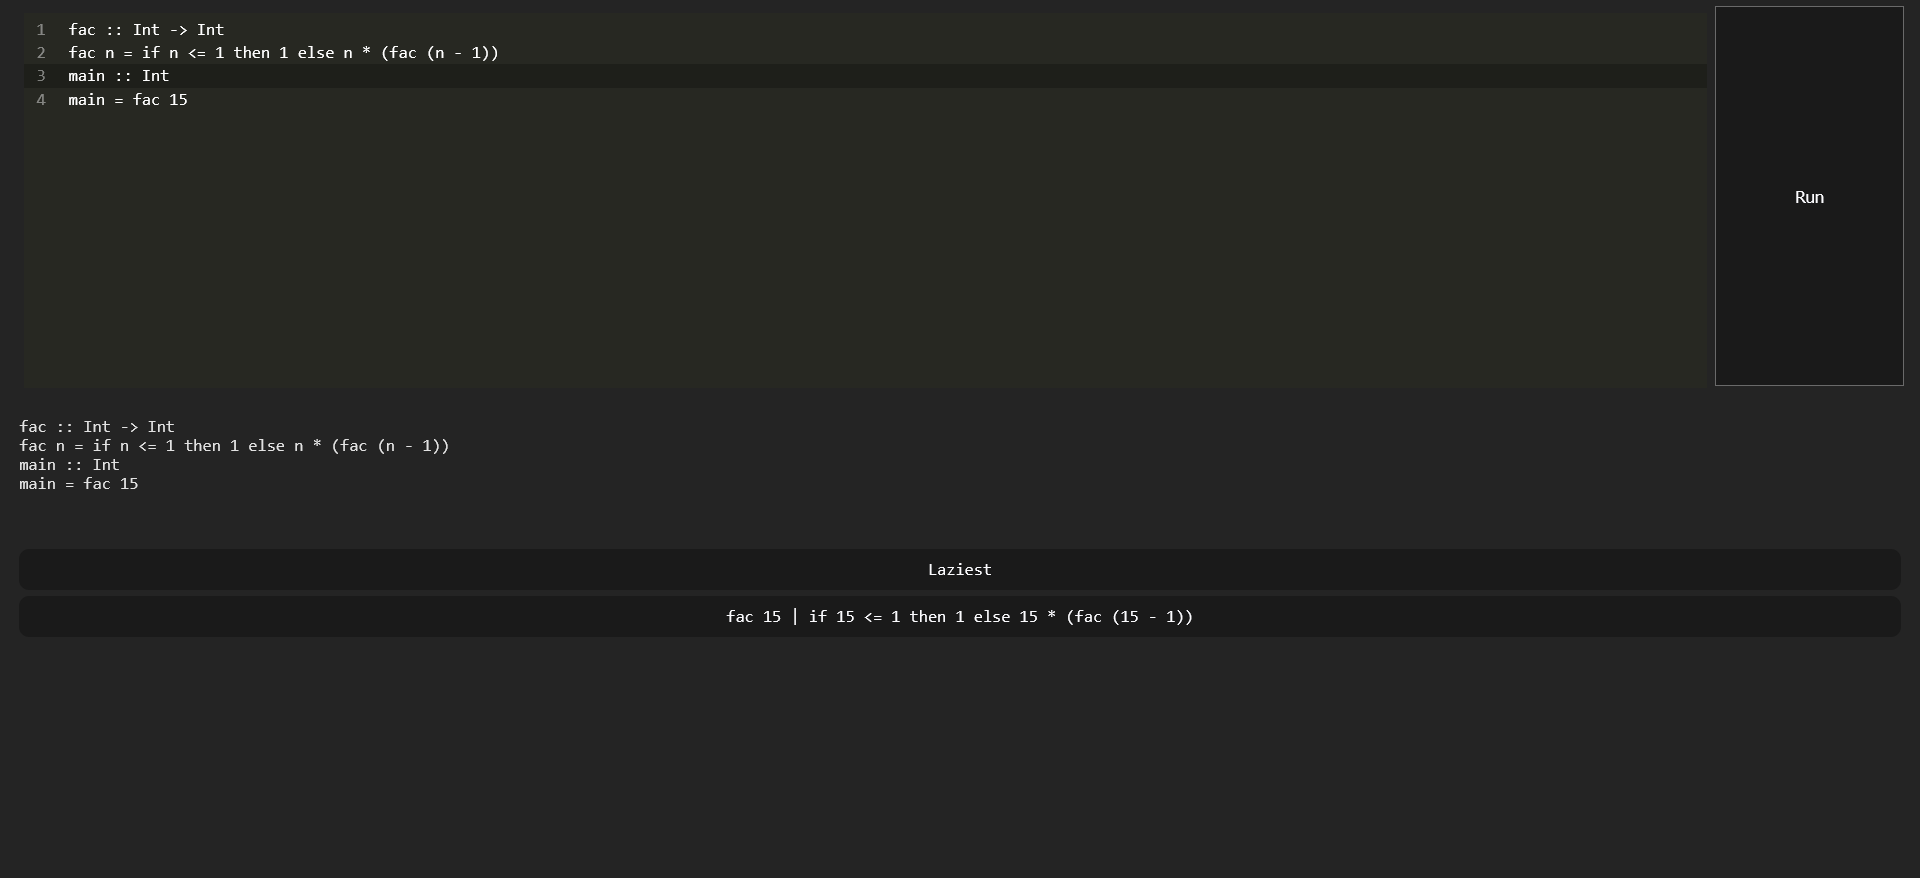
\includegraphics[width=1\linewidth]{images/cycle-1-end.png}
    \caption{The Web UI MVP, as presented to my client at the end of cycle 1. Note that this does have type assignments, but these were just ignored by the parser and typechecker at this stage. }
    \label{fig:screenshot_cycle_1_end}
\end{figure}
\section{Testathon}

\begin{figure}[h]
    \centering
    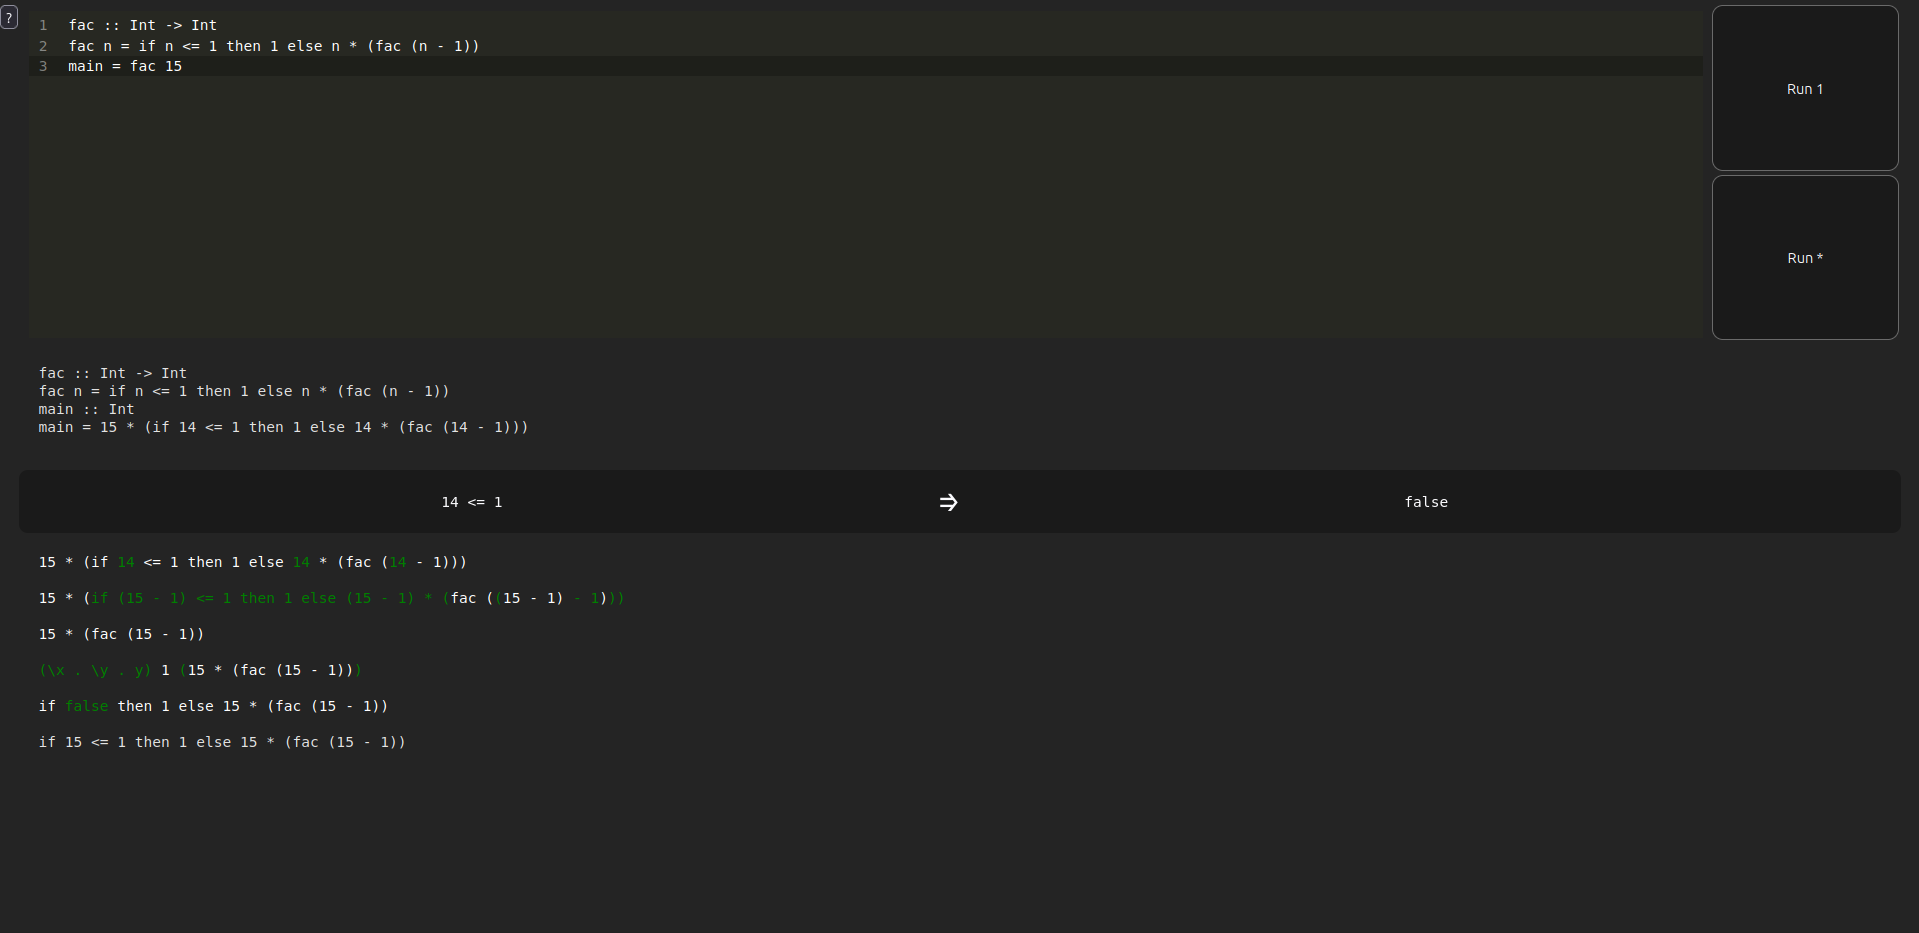
\includegraphics[width=1\linewidth]{images/product_at_testathon.png}
    \caption{The UI as tested in the testathon}
    \label{fig:screenshot_testathon}
\end{figure}

\begin{figure}
    \centering
    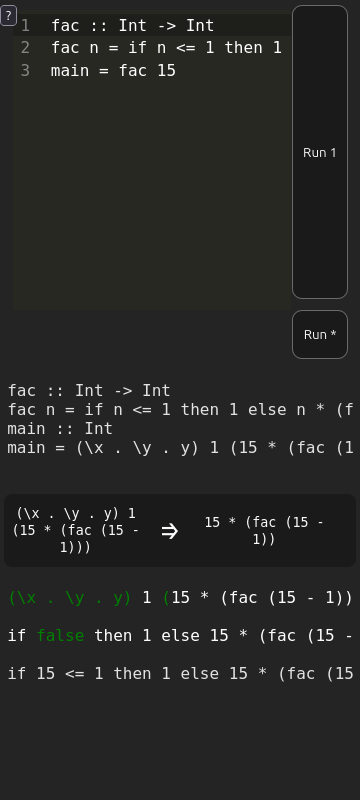
\includegraphics[width=0.5\linewidth]{images/testathon-mobile.png}
    \caption{The UI as tested in the testathon, as it would have appeared on a Samsung Galaxy S20}
    \label{fig:screenshot_testathon_mobile}
\end{figure}

\begin{figure}
    \centering
    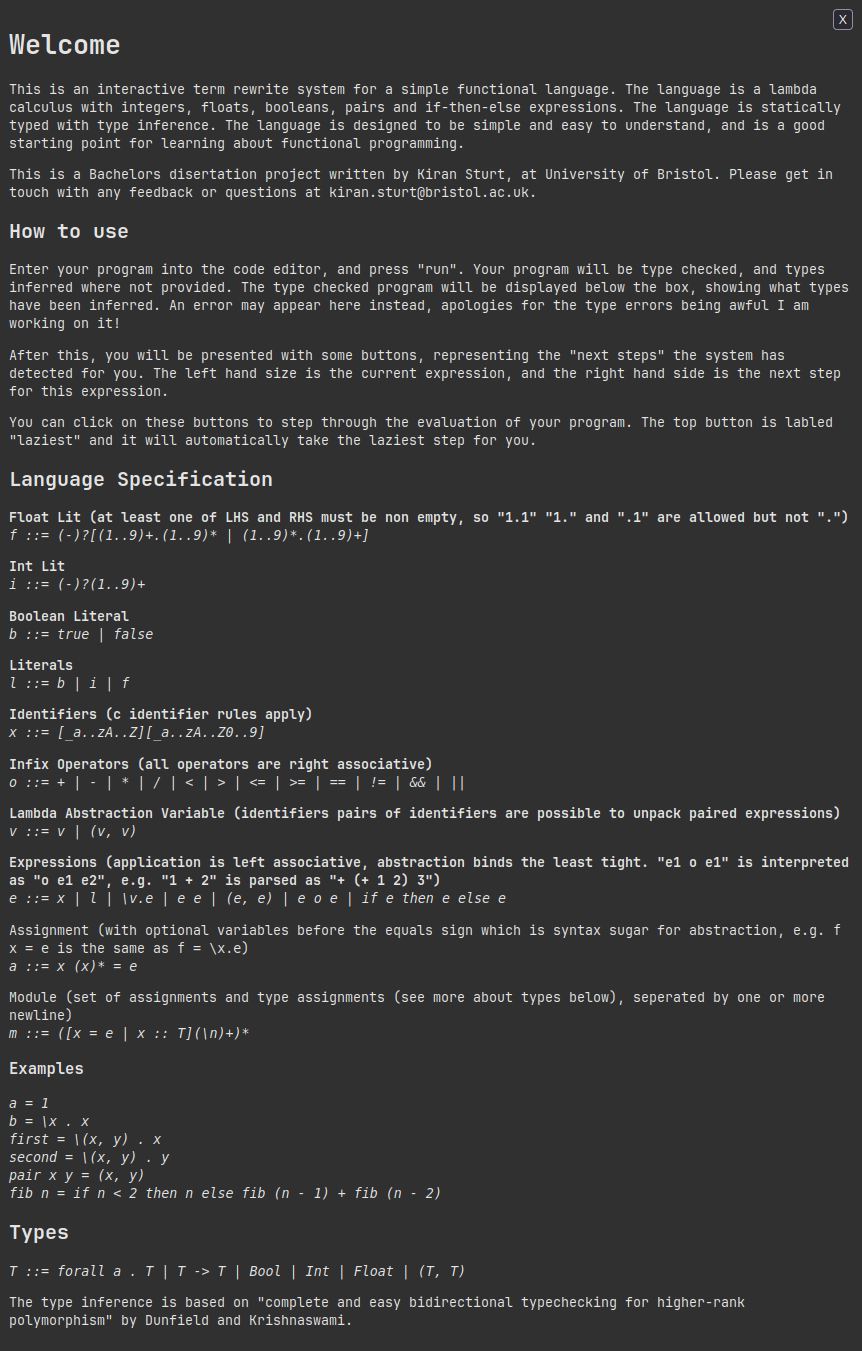
\includegraphics[width=0.9\linewidth]{images/testathon_help_menu_cropped.png}
    \caption{The "Help menu" in the testathon. This was spawned by pressing the "?" button in the top left of the UI, and dismissed by pressing the "X" button, or clicking outside of the box}
    \label{fig:screenshot_testathon_2}
\end{figure}

\chapter{Type System}
\def\OPTIONConf{1}
\linespread{1}

\renewcommand{\mathstrut}{\rule[-1pt]{0pt}{2pt}}

\def\OPTIONLoudLabels{0}
\def\OPTIONArxiv{1}

\definecolor{dHilite}{rgb}{0.9, 0.9, 0.6}
\definecolor{dRed}{rgb}{0.65, 0.0, 0.0}
\definecolor{dGreen}{rgb}{0.0, 0.65, 0.0}
\definecolor{dDkGreen}{rgb}{0.0, 0.35, 0.0}
\definecolor{dBlue}{rgb}{0.0, 0.0, 0.65}
\definecolor{dPurple}{rgb}{0.65, 0.0, 0.65}
\definecolor{dDigPurple}{rgb}{0.5, 0.0, 0.5}
\definecolor{dFaint}{rgb}{0.7, 0.7, 0.7}
\definecolor{dGray}{rgb}{0.5, 0.5, 0.5}
\definecolor{dDark}{rgb}{0.2, 0.2, 0.2}
\definecolor{dAlmostBlack}{rgb}{0.1, 0.1, 0.1}

\makeatletter
\def\url@MGstyle{%
\def\UrlFont{\tiny\huge\ttfamily}%
%
%
\Url@do
}
\makeatother
%
%
\newcommand{\marginPseudoURL}[1]{\tt #1}
\newcommand{\marginnote}[1]{\marginparwidth=40pt \marginpar{%
    \raisebox{-2ex}{\parbox{40pt}{\raggedright\scriptsize #1}}}}

\makeatletter
\def\url@vttstyle{%
  \@ifundefined{selectfont}{\def\UrlFont{\tt}}{\def\UrlFont{\normalfont\fontfamily{cmvtt}\selectfont}}}
\makeatother
%
\urlstyle{vtt}

%
%
%
%
%
%

\newcommand\textvtt[1]{{\normalfont\fontfamily{cmvtt}\selectfont #1}}

\newcommand{\LoudLabel}[1]{\idempotentlabel{#1}%
\ifnum\OPTIONLoudLabels=1%
  \ifnum\OPTIONConf=1%
  \marginnote{\tiny\textvtt{#1}}%
  \else%
  \marginnote{\textvtt{#1}}%
  \fi%
\fi%
}

\newcommand{\idempotentlabel}[1]{%
    \ifcsname IDEMPFLAG#1\endcsname%
      %
      \message{YYY ALREADY DEFINED: #1}
    \else%
      %
      \message{YYZ NOT ALREADY DEFINED: #1}
      \expandafter\gdef\csname IDEMPFLAG#1\endcsname{d}%
      %
      \label{#1}%
    \fi}

%

%
\ifnum\OPTIONLoudLabels=1%
\newcommand{\Label}[1]{\LoudLabel{#1}}%
\newcommand{\FLabel}[1]{\idempotentlabel{#1}%
{\tt\scriptsize{#1}}}%
\else%
\newcommand{\Label}[1]{\idempotentlabel{#1}}%
\newcommand{\FLabel}[1]{\idempotentlabel{#1}}%
\fi

%
%
%
%
%
%
%
%
\newdimen\zzfontsz
\newcommand{\fontsz}[2]{\zzfontsz=#1%
{\fontsize{\zzfontsz}{1.2\zzfontsz}\selectfont{#2}}}

\newcommand{\texfontsz}[1]{\zzfontsz=#1%
\fontsize{\zzfontsz}{1.25\zzfontsz}\selectfont}

\newcommand{\mathsz}[2]{\text{\fontsz{#1}{$#2$}}}

\newcommand{\XX}{\text{\ding{55}}}
\newcommand{\redXX}{\text{\textcolor{dRed}{\XX}}}
\newcommand{\greencheck}{\text{\textcolor{dGreen}{\checkmark}}}

\newcommand{\fixme}[1]{\textcolor{red}{\texttt{FIXME: {#1}}}}

\newcommand{\flaming}[1]{\textcolor{red}{\fontsz{18pt}{\bf #1}}}
\newcommand{\flamingmath}[1]{\textcolor{red}{\fontsz{18pt}{\bf \ensuremath{#1}}}}

\newcommand{\semiflaming}[1]{\textcolor{dRed}{\sl #1}}

% \newcommand{\mathcolor}[2]{\text{\textcolor{#1}{\ensuremath{#2}}}}

%
\newcommand{\smallblacktriangle}{\text{\textscale{0.7}{$\blacktriangleright$}}}

\newcommand{\setof}[1]{\left\{#1\right\}}
\newcommand{\comprehend}[2]{\setof{{#1} \;\middle|\; {#2}}}

\newcommand{\assign}{\ensuremath{\,{:=}\,}}

\newcommand{\arr}{\rightarrow}
%
%
\def\CompactJudgments{0}
\newcommand{\entails}{\mathrel{\ifnum\CompactJudgments=1%
    \vdash%
  \else%
     \vdash\,%
  \fi}}
\newcommand{\ctxoutsym}{\ifnum\CompactJudgments=1%
    \dashv%
  \else%
     \,\dashv%
  \fi}
\newcommand{\ctxout}[1]{\mathrel{\ctxoutsym}{#1}}

%
\newcommand{\J}{\mathcal{J}}
\newcommand{\judg}{\J}

\newcommand{\MonnierCommaSym}{{\smallblacktriangle}}
\newcommand{\MonnierComma}[1]{{\MonnierCommaSym}_{#1}}

\newcommand{\FV}[1]{\mathrm{FV}(#1)}
\newcommand{\xfev}{\mathsf{FEV}}
\newcommand{\fev}[1]{\xfev(#1)}
\newcommand{\FEV}[1]{\fev{#1}}
\newcommand{\xfsolev}{\mathsf{FSolEV}}
\newcommand{\fsolev}[2]{\xfsolev_{#1}(#2)}

\newcommand{\beeq}{=_{\beta\eta}}

\newcommand{\kindstar}{\star}
\newcommand{\kindnat}{\mathbb{N}}

\newcommand{\inversefn}[1]{{#1}^{-1}}

\newcommand{\emptysig}{\cdot}
\newcommand{\emptyctx}{\cdot}

\newcommand{\natzero}{\mathsf{zero}}
\newcommand{\xnatsucc}{\mathsf{succ}}
\newcommand{\natsucc}[1]{\xnatsucc\texttt{(}{#1}\texttt{)}}


\newcommand{\instantiate}[1]{{#1}\texttt{[-]}}
\newcommand{\quantify}[1]{\Lambda{#1}.\,}


\newcommand{\exvar}[1]{\widehat{#1}}
\newcommand{\exalpha}{\exvar{\alpha}}
\newcommand{\exbeta}{\exvar{\beta}}

\newcommand{\alln}[1]{\forall{#1}{:}\kindnat.\,}

\newcommand{\Match}[2]{{#1} \Rightarrow {#2}}
\newcommand{\matchor}{\ensuremath{\normalfont\,\texttt{|}\hspace{-5.35pt}\texttt{|}\,}}
\newcommand{\ind}[3]{\mathsf{ind}\texttt{(}\Match{\natzero}{#1}%
                     \texttt{,\;}%
                     \Match{\natsucc{#2}}{#3}
                     \texttt{)}}

\newcommand{\exunk}[2]{{#1} : {#2}}
\newcommand{\exsol}[3]{{#1} : {#2} \texttt{=} {#3}}
\newcommand{\exsolnokind}[2]{{#1} \texttt{=} {#2}}
\newcommand{\exsolwild}[2]{({#1} : {#2}\dots)}
\newcommand{\rexvar}[2]{\exsolnokind{#1}{#2}}

\newcommand{\tyname}[1]{\textsf{\normalfont #1}}
%
\newcommand{\unitexp}{\text{\normalfont \tt()}}
\newcommand{\unitty}{\tyname{1}}

\newcommand{\trientails}{\mathrel{{\rhd}\,}}
\newcommand{\trictxoutsym}{{\lhd}}
\newcommand{\trictxout}[1]{\mathrel{\trictxoutsym}{#1}}

\newcommand{\subtypingycolor}[1]{\textcolor{dDigPurple}{#1}}
%
\newcommand{\subtype}{\mathrel{\normalfont\texttt{\subtypingycolor{<:}}}}  %
\newcommand{\declsubtype}{\mathrel{\leq}}

\newcommand{\etal}{{et al.}}
\newcommand{\eg}{e.g.\ }
\newcommand{\ie}{i.e.\ }
\newcommand{\ala}{\`a la\ }
\newcommand{\Wlog}{w.l.o.g.\ }
\newcommand{\visavis}{vis-\`a-vis\ }
\newcommand{\Ocaml}{{OCaml}\xspace}
\newcommand{\OCaml}{\Ocaml}

\newcommand{\naive}{na\"ive\xspace}
\newcommand{\Backslash}{\char"5C}
\newcommand{\Lbrack}{\char"5B}
\newcommand{\Rbrack}{\char"5D}
\newcommand{\Lbrace}{\char"7B}
\newcommand{\Rbrace}{\char"7D}

\newcommand{\Appendixref}[1]{Appendix \ref{#1}}
\newcommand{\Figureref}[1]{Figure \ref{#1}}
\newcommand{\Figref}[1]{Fig.\ \ref{#1}}
\newcommand{\Sectionref}[1]{Section \ref{#1}}
\newcommand{\Secref}[1]{Sec.\ \ref{#1}}
\newcommand{\Chapterref}[1]{Chapter \ref{#1}}

\newcommand{\Listingref}[1]{Listing \ref{#1}}

\newcommand{\Theoremref}[1]{Theorem \ref{#1}}
\newcommand{\Thmref}[1]{Thm.\ \ref{#1}}
\newcommand{\Corollaryref}[1]{Corollary \ref{#1}}
\newcommand{\Corref}[1]{Cor.\ \ref{#1}}
\newcommand{\Lemmaref}[1]{Lemma \ref{#1} (\nameref{#1})}   %
\newcommand{\Lemref}[1]{\Lemma \ref{#1}}   %
%
\newcommand{\Conjectureref}[1]{Conjecture \ref{#1}}
\newcommand{\Propositionref}[1]{Proposition \ref{#1}}
\newcommand{\Propertyref}[1]{Property \ref{#1}}
\newcommand{\Remarkref}[1]{Remark \ref{#1}}
\newcommand{\Tableref}[1]{Table \ref{#1}}

\newcommand{\Definitionref}[1]{Definition \ref{#1}}
\newcommand{\Defnref}[1]{Def.\ \ref{#1}}

%
\newcommand{\ProofCaseRule}[1]{\item \textbf{Case }\textrm{{#1}}: ~ }
\newcommand{\ProofCaseThing}[1]{\ProofCaseRule{\ensuremath{#1}}}
\newcommand{\ProofCasesRules}[1]{\item \textbf{Cases }\textrm{{#1}}: ~ }
\newcommand{\ProofCaseRuleNoColon}[1]{\item \textbf{Case }\textrm{{#1}}}

\gdef\xxDerivationProofCaseColor{N}
\newcommand{\Begincolorcases}[1]{\gdef\xxDerivationProofCaseColor{#1}}
\newcommand{\Endcolorcases}{\gdef\xxDerivationProofCaseColor{N}}

%
%
%
%
%
%
%
%
%
%
%
%
%
%
%
%
%
%
%
%
%
%
%
\newcommand{\DerivationProofCase}[3]{%
     \smallskip
     \item %
       \parbox[t]{100ex}{%
       \textbf{Case } \\[-0.5em]
       $~$\hspace{5ex}
       \if\xxDerivationProofCaseColor N%
           \ensuremath{%
              \Infer{#1}{#2}{#3}%
            }
       \else%
           \colorbox{\xxDerivationProofCaseColor}{%
              \ensuremath{%
                \Infer{#1}{#2}{#3}%
              }%
           }%
        \fi%
     }%
     \nopagebreak \\[-0.8ex]
  }

\newcommand{\DoubleDerivationProofCase}[6]{%
     \smallskip
     \item %
       \parbox[t]{100ex}{%
       \textbf{Case } \\[-0.5em]
       $~$\hspace{5ex}
       \if\xxDerivationProofCaseColor N%
           \ensuremath{%
              \Infer{#1}{#2}{#3}%
              ~~~~~
              \Infer{#4}{#5}{#6}%
            }
       \else%
           \colorbox{\xxDerivationProofCaseColor}{%
              \ensuremath{%
                \Infer{#1}{#2}{#3}%
                ~~~~~
                \Infer{#4}{#5}{#6}%
              }%
           }%
        \fi%
     }%
     \nopagebreak \\[-0.8ex]
  }

\newcommand{\Dee}{\mathcal{D}}
\newcommand{\D}{\mathcal{\Dee}}

\newenvironment{displ}{\vspace{1pt} \begin{center} ~\!\!}{\end{center}}
\newenvironment{mathdispl}{\vspace{1pt} \begin{center} ~\!\!\(}{\)\end{center}}

\newenvironment{ctabular}{%
      \renewcommand{\arraystretch}{1}%
         \vspace{1pt}%
         \begin{center} ~\!\!%
           \begin{tabular}[t]{l}%
     }{%
            \end{tabular}%
          \end{center}%
      }

\newcommand{\arrayenv}[1]{\renewcommand{\arraystretch}{1} \begin{array}[t]{@{}c@{}}#1\end{array}}
\newcommand{\arrayenvc}[1]{\renewcommand{\arraystretch}{1} \begin{array}[c]{@{}c@{}}#1\end{array}}
\newcommand{\arrayenvcl}[1]{\renewcommand{\arraystretch}{1} \begin{array}[c]{@{}l@{}}#1\end{array}}
\newcommand{\arrayenvr}[1]{\renewcommand{\arraystretch}{1} \begin{array}[t]{@{}r@{}}#1\end{array}}
\newcommand{\arrayenvbr}[1]{\renewcommand{\arraystretch}{1} \begin{array}[b]{@{}r@{}}#1\end{array}}
\newcommand{\arrayenvl}[1]{\renewcommand{\arraystretch}{1} \begin{array}[t]{@{}l@{}}#1\end{array}}
\newcommand{\arrayenvb}[1]{\renewcommand{\arraystretch}{1}  \begin{array}[b]{@{}c@{}}#1\end{array}} 
\newcommand{\arrayenvbl}[1]{\renewcommand{\arraystretch}{1}  \begin{array}[b]{@{}l@{}}#1\end{array}}
\newcommand{\arrayenvblll}[1]{\renewcommand{\arraystretch}{1}  \begin{array}[b]{@{}lll@{}}#1\end{array}}
\newcommand{\pfarr}[1]{\begin{array}[b]{@{}l@{}}#1\end{array}}

%
\newcommand{\BeginProof}{\renewcommand{\arraystretch}{1.1} \begin{tabular}[b]{r@{}r @{} l  l}}
\newcommand{\EndProof}{\end{tabular} \renewcommand{\arraystretch}{\mydefaultarraystretch}}

\newcommand{\Hand}{\text{\Pointinghand~~~~}}

\newcommand{\Pf}[4] {&$#1$ $#2$\, & $#3$ & #4 \\}
\newcommand{\Pfmrg}[3] {&$#1$\, & $#2$ & #3 \\}
\newcommand{\stepPf}[3] {\Pf{#1}{\,\step\,}{#2}{#3}}
\newcommand{\EPf}[3] {\Pf{#1}{\Entails}{#2}{#3}}
\newcommand{\LetPf}[3] {\Pf{\text{Let}\,~{#1}}{=\,}{#2\text{.}}{#3}}
\newcommand{\ForallPf}[3] {\Pf{\text{For all}\,~{#1}}{\in\,}{#2}{#3}}
\newcommand{\mkpf}[4] {\Pf{#2}{#1\,}{#3}{#4}}

\newcommand{\ePf}[3] {\mkpf{\entails}{#1}{#2}{#3}}
\newcommand{\eqPf}[3] {\mkpf{=}{#1}{#2}{#3}}
\newcommand{\continueeqPf}[2] {\mkpf{=}{~}{#1}{#2}}
\newcommand{\rightstarteqPf}[1] {\mkpf{~}{~}{#1}{~}}
\newcommand{\neqPf}[3] {\mkpf{\neq}{#1}{#2}{#3}}
\newcommand{\ltPf}[3] {\mkpf{<}{#1}{#2}{#3}}
\newcommand{\leqPf}[3] {\mkpf{\leq}{#1}{#2}{#3}}
\newcommand{\inPf}[3] {\mkpf{\in}{#1}{#2}{#3}}
\newcommand{\notinPf}[3] {\mkpf{\notin}{#1}{#2}{#3}}

\newcommand{\trailingjust}[1]{\Pf{}{}{}{~~{#1}}}
\newcommand{\derivesPf}[1]{${#1} \derives~~$}

\newcommand{\contraPf}[1] {%
          \Pf{\Rightarrow\Leftarrow}{}{} {}%
          \Pf{#1}{}{} {By contradiction}%
       }

\newcommand{\NOTePf}[3] {\Pf{#1}{\not\entails\;}{#2}{#3}}
\newcommand{\proofsep}{\,\\[-0.5em]}
\newcommand{\PfTwo}[7]{\Pf{\arrayenvr{{#1}\\{#4}}}{\arrayenvl{{#2}\\{#5}}}{\arrayenvl{{#3}\\{#6}}}%
                                              {\drophalf{\!\ensuremath{\left\} \begin{array}{r l} \,\\ \, \end{array}\!\!\!\!\!%
                                                      \text{#7} \right.}}}}
\newenvironment{llproof}{\BeginProof}{\EndProof}
\newcommand{\decolumnizePf}{\end{llproof} ~\\ \begin{llproof}}

%
\newcommand{\proofheading}[1]{}  %

\newcommand{\ditto}{\ensuremath{''}}


\newcommand{\xdom}{\mathsf{dom}}
\newcommand{\dom}[1]{\xdom(#1)}

\newcommand{\xweight}{\mathsf{weight}}
\newcommand{\weight}[2]{\xweight_{#1}(#2)}

\newcommand{\xangst}{\mathsf{angst}}
\newcommand{\angst}[2]{\xangst_{#1}(#2)}

\newcommand{\xunsol}{\mathsf{unsol}}
\newcommand{\unsol}[2]{\xunsol_{#1}(#2)}

\newcommand{\xunsolved}{\mathsf{unsolved}}
\newcommand{\unsolved}[1]{\xunsolved(#1)}

\newcommand{\xGtypesize}[1]{\mathsf{size}_{#1}}
\newcommand{\Gtypesize}[2]{\xGtypesize{#1}(#2)}

\newcommand{\union}{\mathrel{\cup}}
\newcommand{\sect}{\mathrel{\cap}}


\newcommand{\normalize}{\mathrel{\Downarrow}}


%
%
\newcommand{\textgraybox}[1]{\boxed{#1}}
\newcommand{\graybox}[1]{\textgraybox{\ensuremath{#1}}}

\newcommand{\tightcolorbox}[2]{\setlength{\fboxsep}{1pt}\colorbox{#1}{#2}}

%
\newcommand{\textcolorbox}[2]{\tightcolorbox{#1}{#2}}
\newcommand{\textshadebox}[1]{\textcolorbox{grayboxgray}{#1}}
%
\newcommand{\shadebox}[1]{\text{\textshadebox{\ensuremath{#1}}}}

%

%
\newcommand{\mathcolorbox}[2]{\text{\tightcolorbox{#1}{$\displaystyle {#2}$}}}

%
%
%
%

\newcommand{\judgboxfontsize}[1]{%
    \ifnum\OPTIONConf=1%
        \mathsz{11pt}{#1}%
    \else%
        \mathsz{14pt}{#1}%
    \fi}
\newcommand{\judgbox}[2]{%
      {\raggedright \textgraybox{\ensuremath{\judgboxfontsize{#1}}}\!%
        \fontsz{9pt}{\begin{tabular}[c]{l} #2 \end{tabular}} %
}}


\newcommand{\bnfas}{\mathrel{::=}}
\newcommand{\bnfalt}{\mathrel{\mid}}

\newcommand{\derives}{\mathrel{::}}

\newcommand{\AllSym}{\forall}
\newcommand{\xAll}[1]{\AllSym#1}
\newcommand{\All}[1]{\xAll{#1}.\:}

\newcommand{\AND}{\text{~~and~~}}

\newcommand{\Infer}[3]{\inferrule*[right={\text{\strut#1}}]{{}#2\mathstrut}{{}#3\mathstrut}}




\newcommand{\keyword}[1]{\textsf{#1}}
\newcommand{\textkw}[1]{\keyword{#1}}
\newcommand{\lam}[1]{\lambda #1.\,}
\newcommand{\fun}[2]{\lam{#1}{#2}}
\newcommand{\typelam}[1]{\Lambda #1.\,}
\newcommand{\LAM}[1]{\typelam{#1}}
\newcommand{\Let}[2]{\textkw{let}\;{#1}\,\texttt{=}\,{#2}\;\textkw{in}\;}

\newcommand{\bigprec}{\mathrel{\mathsz{14pt}{\prec}}}


\newcommand{\atomic}[1]{{#1}\;\mathrm{atomic}}

\newcommand{\declsubjudg}[3]{\ensuremath{{#1} \entails {#2} \declsubtype {#3}}}
\newcommand{\typejudg}[3]{\ensuremath{{#1} \entails {#2} : {#3}}}
\newcommand{\subjudg}[4]{\ensuremath{{#1} \entails {#2} \subtype {#3} \ctxout{#4}}}

%
%
\newdimen\zzinstsymLTwidth
\newdimen\zzinstsymEQwidth
\newdimen\zzinstsymDiff
\newcommand{\instsymLeq}{%
    \settowidth{\zzinstsymLTwidth}{\text{\normalfont\tt<}}%
    \settowidth{\zzinstsymEQwidth}{\text{\normalfont=}}%
    \setlength{\zzinstsymDiff}{\zzinstsymEQwidth}%
    \addtolength{\zzinstsymDiff}{-\zzinstsymLTwidth}%
    \text{\raisebox{-0.22ex}{\normalfont=}%
%
    \hspace{-\zzinstsymEQwidth}%
    \hspace{0.5\zzinstsymDiff}%
    \raisebox{0.77ex}{\normalfont\tt<}}}
\newcommand{\instsymColon}{%
     \raisebox{-0.09ex}{\text{\normalfont{:}}}}
%
%
%
\newcommand{\instsyml}{\subtypingycolor{\instsymColon\hspace{0.05ex}\instsymLeq}}
\newcommand{\instsymr}{\subtypingycolor{\instsymLeq\hspace{0.05ex}\instsymColon}}
\newcommand{\instsymlop}{\mathrel{\instsyml}}
\newcommand{\instsymrop}{\mathrel{\instsymr}}

\newcommand{\instjudg}[4]{\ensuremath{{#1} \entails {#2} \instsymlop {#3} \ctxout{#4}}}
\newcommand{\instjudgr}[4]{\ensuremath{{#1} \entails {#3} \instsymrop {#2} \ctxout{#4}}}

\newcommand{\declsubjudgPf}[4] {\Pf{#1}{\entails}{{#2} \declsubtype {#3}}{#4}}
\newcommand{\subjudgPf}[5] {\Pf{#1}{\entails}{{#2} \subtype {#3} \ctxout{#4}}{#5}}
\newcommand{\substextendPf}[3] {\Pfmrg{{#1} \extendssym\,}{#2}{#3}}
\newcommand{\instjudgPf}[5]{\Pf{#1}{\entails}{{#2} {\;\instsyml\;} {#3} \ctxout{#4}}{#5}}
\newcommand{\instjudgrPf}[5]{\Pf{#1}{\entails}{{#3} {\;\instsymr\;} {#2} \ctxout{#4}}{#5}}

\newcommand{\chkcolor}{dBlue}
\newcommand{\syncolor}{dRed}
\newcommand{\appcolor}{dDkGreen}
\newcommand{\chk}{\mathrel{\mathcolor{\chkcolor}{\Leftarrow}}}
\newcommand{\uncoloredsyn}{{\Rightarrow}}
\newcommand{\syn}{\mathrel{\mathcolor{\syncolor}{\uncoloredsyn}}}
\newcommand{\appsep}{\;{\mathcolor{\appcolor}{\bullet}}\;}
%
\newcommand{\app}{\mathrel{\mathcolor{\appcolor}{{\uncoloredsyn}\hspace{-1.2ex}{\uncoloredsyn}}}}

\newcommand{\chkjudg}[4]{\ensuremath{{#1} \entails {#2} \chk {#3} \ctxout{#4}}}
\newcommand{\appjudg}[5]{\ensuremath{{#1} \entails {#3} \appsep {#2} \app {#4} \ctxout{#5}}}
\newcommand{\synjudg}[4]{\ensuremath{{#1} \entails {#2} \syn {#3} \ctxout{#4}}}

\newcommand{\declchkjudg}[3]{\ensuremath{{#1} \entails {#2} \chk {#3}}}
\newcommand{\declappjudg}[4]{\ensuremath{#1} \entails {#3} \appsep {#2}  \app {#4}}
\newcommand{\declsynjudg}[3]{\ensuremath{{#1} \entails {#2} \syn {#3}}}

\newcommand{\chkjudgPf}[5]{\Pf{#1}{\entails}{{#2} \chk {#3} \ctxout{#4}}{#5}}
\newcommand{\appjudgPf}[6]{\Pf{#1}{\entails}{{#3} \appsep {#2} \app {#4} \ctxout{#5}}{#6}}
\newcommand{\synjudgPf}[5]{\Pf{#1}{\entails}{{#2} \syn {#3} \ctxout{#4}}{#5}}
\newcommand{\declchkjudgPf}[4]{\Pf{#1}{\entails}{{#2} \chk {#3}}{#4}}
\newcommand{\declappjudgPf}[5]{\Pf{#1}{\entails}{{#3} \appsep {#2} \app {#4}}{#5}}
\newcommand{\declsynjudgPf}[4]{\Pf{#1}{\entails}{{#2} \syn {#3}}{#4}}


\newcommand{\hyp}[2]{{#1}:{#2}}
\newcommand{\hypeq}[2]{{#1} = {#2}}
\newcommand{\tighthypeq}[2]{{#1}{=}{#2}}
%
\newcommand{\alltype}[1]{\All{#1}}
\newcommand{\num}{\mathsf{int}}
\newcommand{\bool}{\mathsf{bool}}

\newcommand{\grow}[2]{{#1} \sqsupseteq {#2}}

\newcommand{\idsubst}{\mathsf{id}}

\newcommand{\extendssym}{\longrightarrow}
\newcommand{\extends}[2]{{#1} \extendssym {#2}}
%
\newcommand{\substextend}[2]{\extends{#1}{#2}}

\newcommand{\judgetp}[2]{{#1} \entails {#2}}
\newcommand{\judgetpPf}[3]{\Pf{#1}{\entails}{#2}{#3}}
%
%
\newcommand{\typesize}[2]{|{#1} {\;\entails} {#2}|}

\newcommand{\judgectx}[1]{{#1}~\mathit{ctx}}
\newcommand{\judgectxPf}[2]{\Pf{}{}{\judgectx{#1}}{#2}}

\newcommand{\xcompletes}{\ensuremath{\mathsf{completes}}}
\newcommand{\xcompletedby}{\ensuremath{\mathsf{completed\;by}}}
%
\newcommand{\completedby}[2]{{#1} \;\flamingmath{\xcompletedby}\; {#2}}
\newcommand{\apply}[2]{{[{#1}]}{#2}}

\newcommand{\ahat}{\hat{\alpha}}
\newcommand{\bhat}{\hat{\beta}}
\newcommand{\chat}{\hat{\gamma}}
\newcommand{\dhat}{\hat{\delta}}

%
%
%
\newcommand{\hsubst}[5]{[{#2}/{#3}]^{#1}_{#2}{#4}}

%
%
%
\newcommand{\rulename}[1]{\text{\normalfont\textsf{#1}}}

%
%
%
\newcommand{\substextendrulename}[1]{\ensuremath{{\extendssym}{\rulename{#1}}}\xspace}
\newcommand{\substextendId}{\substextendrulename{ID}}

\newcommand{\substextendUU}{\substextendrulename{Uvar}}
\newcommand{\substextendVV}{\substextendrulename{Var}}
\newcommand{\substextendEE}{\substextendrulename{Unsolved}}
\newcommand{\substextendSolSol}{\substextendrulename{Solved}}
\newcommand{\substextendMonMon}{\substextendrulename{Marker}}

\newcommand{\substextendSolve}{\substextendrulename{Solve}}
\newcommand{\substextendAdd}{\substextendrulename{Add}}
\newcommand{\substextendAddSolved}{\substextendrulename{AddSolved}}


%
%
%
\newcommand{\Dsubrulename}[1]{\ensuremath{{\declsubtype}\rulename{#1}}\xspace}
\newcommand{\DsubVar}{\Dsubrulename{Var}}
\newcommand{\DsubUnit}{\Dsubrulename{Unit}}
\newcommand{\DsubArr}{\Dsubrulename{\ensuremath{\arr}}}
\newcommand{\DsubImp}{\DsubArr} %
\newcommand{\DsubAllL}{\Dsubrulename{\ensuremath{\forall}{L}}}
\newcommand{\DsubAllR}{\Dsubrulename{\ensuremath{\forall}{R}}}

%
%
%
\newcommand{\Subrulename}[1]{\ensuremath{{\subtype}\rulename{#1}}\xspace}
\newcommand{\SubVar}{\Subrulename{Var}}
\newcommand{\SubUnit}{\Subrulename{Unit}}
\newcommand{\SubExvar}{\Subrulename{Exvar}}
\newcommand{\SubArr}{\Subrulename{\ensuremath{\arr}}}
\newcommand{\SubImp}{\SubArr} %
\newcommand{\SubAllL}{\Subrulename{\ensuremath{\forall}{L}}}
\newcommand{\SubAllR}{\Subrulename{\ensuremath{\forall}{R}}}

\newcommand{\SubSubst}[1]{\Subrulename{\flaming{Subst{#1}}}}
\newcommand{\SubSubstL}{\SubSubst{L}}
\newcommand{\SubSubstR}{\SubSubst{R}}

\newcommand{\SubInst}[1]{\Subrulename{Instantiate{#1}}}
\newcommand{\SubInstL}{\SubInst{L}}
\newcommand{\SubInstR}{\SubInst{R}}

%
%
%
\newcommand{\DeclWFrulename}[1]{\ensuremath{\rulename{Decl{#1}WF}}\xspace}
\newcommand{\DeclUvarWF}{\DeclWFrulename{Uvar}}
\newcommand{\DeclUnitWF}{\DeclWFrulename{Unit}}
\newcommand{\DeclArrowWF}{\DeclWFrulename{Arrow}}
\newcommand{\DeclForallWF}{\DeclWFrulename{Forall}}

%
%
%
\newcommand{\WFrulename}[1]{\ensuremath{\rulename{{#1}WF}}\xspace}
\newcommand{\UvarWF}{\WFrulename{Uvar}}
\newcommand{\UnitWF}{\WFrulename{Unit}}
\newcommand{\EvarWF}{\WFrulename{Evar}}
\newcommand{\SolvedEvarWF}{\WFrulename{SolvedEvar}}
\newcommand{\ArrowWF}{\WFrulename{Arrow}}
\newcommand{\ForallWF}{\WFrulename{Forall}}


%
%
%
\newcommand{\CWFrulename}[1]{\ensuremath{\rulename{{#1}Ctx}}\xspace}
\newcommand{\EmptyCWF}{\CWFrulename{Empty}}
\newcommand{\UvarCWF}{\CWFrulename{Uvar}}
\newcommand{\EvarCWF}{\CWFrulename{Evar}}
\newcommand{\SolvedEvarCWF}{\CWFrulename{SolvedEvar}}
\newcommand{\VarCWF}{\CWFrulename{Var}}
\newcommand{\MarkerCWF}{\CWFrulename{Marker}}


%
%
%
\newcommand{\Instrulename}[1]{\ensuremath{\rulename{Inst{#1}}}\xspace}
\newcommand{\InstLrulename}[1]{\Instrulename{L{#1}}}
\newcommand{\InstRrulename}[1]{\Instrulename{R{#1}}}

\newcommand{\InstLSolve}{\InstLrulename{Solve}}
\newcommand{\InstLReach}{\InstLrulename{Reach}}
\newcommand{\InstLArr}{\InstLrulename{Arr}}
\newcommand{\InstLAllR}{\InstLrulename{AllR}}

\newcommand{\InstRSolve}{\InstRrulename{Solve}}
\newcommand{\InstRReach}{\InstRrulename{Reach}}
\newcommand{\InstRArr}{\InstRrulename{Arr}}
\newcommand{\InstRAllL}{\InstRrulename{AllL}}


%
%
%
\newcommand{\CompletesRule}{\rulename{completes}}
%
%
%
%
%
%
%
%




%
%
%
\newcommand{\Decltyrulename}[1]{\ensuremath{\rulename{Decl#1}}\xspace}

\newcommand{\DeclIntrorulename}[1]{\Decltyrulename{\ensuremath{#1}I}}
\newcommand{\DeclIntroSynrulename}[1]{\Decltyrulename{\ensuremath{#1}I$\syn$}}
\newcommand{\DeclElimrulename}[1]{\Decltyrulename{\ensuremath{#1}E}}
\newcommand{\DeclApprulename}[1]{\Decltyrulename{\ensuremath{#1}App}}

%
\newcommand{\DeclVar}{\Decltyrulename{Var}}
\newcommand{\DeclSub}{\Decltyrulename{Sub}}
\newcommand{\DeclAnno}{\Decltyrulename{Anno}}

%
\newcommand{\DeclUnitIntro}{\DeclIntrorulename{\unitty}}
%
\newcommand{\DeclUnitIntroSyn}{\DeclIntroSynrulename{\unitty}}

%
\newcommand{\DeclArrIntro}{\DeclIntrorulename{\arr}}
\newcommand{\DeclArrIntroSyn}{\DeclIntroSynrulename{\arr}}
\newcommand{\DeclArrElim}{\DeclElimrulename{\arr}}

%
\newcommand{\DeclAllIntro}{\DeclIntrorulename{\AllSym}}
%
\newcommand{\DeclAllElim}{\DeclElimrulename{\AllSym}}

\newcommand{\DeclArrApp}{\DeclApprulename{\arr}}
%
\newcommand{\DeclAllApp}{\DeclApprulename{\forall}}
%

%
%
%
\newcommand{\Tyrulename}[1]{\ensuremath{\rulename{#1}}\xspace}

\newcommand{\Introrulename}[1]{\Tyrulename{\ensuremath{#1}I}}
\newcommand{\IntroSynrulename}[1]{\Tyrulename{\ensuremath{#1}I$\syn$}}
\newcommand{\Elimrulename}[1]{\Tyrulename{\ensuremath{#1}E}}
\newcommand{\Apprulename}[1]{\Tyrulename{\ensuremath{#1}App}}

%
\newcommand{\Var}{\Tyrulename{Var}}
\newcommand{\Sub}{\Tyrulename{Sub}}
\newcommand{\Anno}{\Tyrulename{Anno}}

%
\newcommand{\SubstSyn}{\Tyrulename{Subst$\syn$}}
\newcommand{\SubstChk}{\Tyrulename{Subst$\chk$}}

%
\newcommand{\UnitIntro}{\Introrulename{\unitty}}
%
\newcommand{\UnitIntroSyn}{\IntroSynrulename{\unitty}}

%
\newcommand{\ArrIntro}{\Introrulename{\arr}}
\newcommand{\ArrIntroSyn}{\IntroSynrulename{\arr}}
\newcommand{\ArrElim}{\Elimrulename{\arr}}

%
\newcommand{\AllIntro}{\Introrulename{\AllSym}}
%
\newcommand{\AllElim}{\Elimrulename{\AllSym}}

%
\newcommand{\ArrApp}{\Apprulename{\arr}}
%
\newcommand{\AllApp}{\Apprulename{\forall}}
%
\newcommand{\SubstApp}{\Apprulename{\rulename{Subst}}}
%
\newcommand{\SolveApp}{\Apprulename{\ahat}}
%

%
%
%
\newcommand{\subtermofsym}{\preceq}
\newcommand{\subtermof}{\mathrel{\subtermofsym}}
\newcommand{\propersubtermofsym}{\prec}
\newcommand{\propersubtermof}{\mathrel{\propersubtermofsym}}
\newcommand{\subtermofPf}[3] {\mkpf{\subtermof}{#1}{#2}{#3}}
\newcommand{\propersubtermofPf}[3] {\mkpf{\propersubtermof}{#1}{#2}{#3}}
\newcommand{\notsubtermofPf}[3] {\mkpf{\not\subtermof}{#1}{#2}{#3}}
\newcommand{\notpropersubtermofPf}[3] {\mkpf{\not\propersubtermof}{#1}{#2}{#3}}

\newcommand{\occursinsidearrow}{{\hspace{0.6ex}\raisebox{-0.4ex}{%
       \ensuremath{\propersubtermof\rput[b](-1.35ex,1.2ex){\ensuremath{\mathsz{1.4ex}{\arr}}}}}}}
\newcommand{\notoccursinsidearrow}{{\hspace{0.6ex}\raisebox{-0.4ex}{%
       \ensuremath{\propersubtermof{\rput[b](-2.3ex,0.0ex){\ensuremath{\not}}}\rput[b](-1.35ex,1.2ex){\ensuremath{\mathsz{1.4ex}{\arr}}}}}}}

\newcommand{\occursinsidearrowPf}[3] {\mkpf{\!\occursinsidearrow\!}{#1}{#2}{#3}}
\newcommand{\notoccursinsidearrowPf}[3] {\mkpf{\!\notoccursinsidearrow\!}{#1}{#2}{#3}}


%
%
%
\newcommand{\Ctxsubrulename}[1]{\ensuremath{\rulename{CtxSub#1}}\xspace}
\newcommand{\CtxsubEmpty}{\Ctxsubrulename{Empty}}
\newcommand{\CtxsubUvar}{\Ctxsubrulename{Uvar}}
\newcommand{\CtxsubVar}{\Ctxsubrulename{Var}}

%
%
%
\newcommand{\AssignRuleName}[1]{\ensuremath{\rulename{A#1}}\xspace}
\newcommand{\AssignIntroName}[1]{\AssignRuleName{\ensuremath{#1}I}}
\newcommand{\AssignElimName}[1]{\AssignRuleName{\ensuremath{#1}E}}
\newcommand{\AssignVar}{\AssignRuleName{Var}}
\newcommand{\AssignUnit}{\AssignRuleName{Unit}}
\newcommand{\AssignArrIntro}{\AssignIntroName{\arr}}
\newcommand{\AssignArrElim}{\AssignElimName{\arr}}
\newcommand{\AssignAllIntro}{\AssignIntroName{\forall}}
\newcommand{\AssignAllElim}{\AssignElimName{\forall}}
\newcommand{\judge}[3]{{#1} \vdash {#2} : {#3}}

%
%
%
\newcommand{\citepSequentCalculus}{\citep{Gentzen35}}
\newcommand{\citetSequentCalculus}{\citet{Gentzen35}}
\newcommand{\citepSubformulaProperty}{\citep[p.\ 87]{Gentzen35}}
\newcommand{\citetSubformulaProperty}{\citet[p.\ 87]{Gentzen35}}


%
%
%
%
\newcommand{\Fsub}{\ensuremath{{\text{F}}_{\texttt{<:}}}\xspace}

%
\newcommand{\Csharp}{\ensuremath{\text{\textrm{C}}^\sharp}}

%
\newcommand{\MLF}{\ensuremath{\mathsf{ML}^\mathsf{F}}\xspace}


%
%
%
\newcommand{\contextappvar}[2]{{[{#1}]}^\dagger{#2}}
\newcommand{\contextapp}[2]{{[{#1}]{#2}}}

\newcommand{\soln}[1]{\left|{#1}\right|}    %

\newcommand{\equivctxsym}{\simeq}
\newcommand{\equivctx}[2]{{#1} \equivctxsym {#2}}

\newcommand{\LOCALCOPY}[1]{%
          \href{papers/#1}{\bf \textcolor{dGreen}{local copy}}}


\newcommand{\Uniontype}{$\bigcup$}
\newcommand{\Unionname}{\text{Name}}
\newcommand{\Producttype}{$\times$}

\newcommand{\TypeAlias}[2]{[#1 : #2]}

\newcommand{\Aliasrulename}{\Tyrulename{\ensuremath{}Alias}}
\newcommand{\Pairsynthrulename}{\Tyrulename{\Producttype$\syn$}}
\newcommand{\Intsynthrulename}{\Tyrulename{IntLit$\syn$}}
\newcommand{\Boolsynthrulename}{\Tyrulename{BoolLit$\syn$}}
\newcommand{\Matchsynthrulename}{\Tyrulename{Match$\syn$}}

\definecolor{myTcRuleColour}{rgb}{0.8, 0.8, 0.8}
\newcommand{\MyTCRule}[1]{\colorbox{myTcRuleColour}{{#1}}}

\newcommand{\Intsubrulename}{\Subrulename{\Inttype}}
\newcommand{\LAliassubrulename}{\Subrulename{\text{LAlias}}}
\newcommand{\RAliassubrulename}{\Subrulename{\text{RAlias}}}
\newcommand{\Boolsubrulename}{\Subrulename{\Booltype}}
\newcommand{\Pairsubrulename}{\Subrulename{\Producttype}}
\newcommand{\Unionsubrulename}{\Subrulename{$\bigcup$}}

\newcommand{\Inttype}{\text{Int}}
\newcommand{\Booltype}{\text{Bool}}
\begin{figure}[h]
  \centering
  \begin{minipage}{0.465\textwidth}
  \[
      \begin{array}{llcl}
      \text{Types} & A, B, C & \bnfas &
            \Inttype \bnfalt \Booltype \bnfalt \alpha \bnfalt \ahat \bnfalt 
            \\[1pt] &&&\!\!\!\;\;\;
            \alltype{\alpha}{A} \bnfalt A \arr B \bnfalt
            % \\[1pt] &&&\!\!\!\;\; \TypeAlias{A}{B} \bnfalt  
            \\[1pt] &&&\!\!\!\;\;
            (A, B) \bnfalt
            \\[1pt] &&&\!\!\!\;\;
            \Unionname[A_1, \dots, A_n]
      \\[2pt]
      \text{Monotypes} & \tau,\sigma & \bnfas &
            \Inttype \bnfalt \Booltype \bnfalt \alpha \bnfalt \ahat \bnfalt 
            \\[1pt] &&&\!\!\!\;\;
            A \arr B \bnfalt (A, B)
            % (A, B) \bnfalt \TypeAlias{A}{B}
        \\[2pt]
      \text{Contexts} & \Gamma, \Delta, \Theta & \bnfas &
                  \cdot
                  \bnfalt \Gamma, \alpha 
                  \bnfalt \Gamma, x:A
                  \\[1pt] &&&\!\!\!\;\;
                  \bnfalt \Gamma, \ahat
                  \bnfalt \Gamma, \hypeq{\ahat}{\tau}
                  \\[1pt] &&&\!\!\!\;\;
                  \bnfalt \Gamma, \MonnierComma{\ahat}
      % \\[2pt] % No need as I am not proving completeness
      % \text{Complete Contexts}     & \Omega & \bnfas &
      %             \cdot
      %             \bnfalt    \Omega, \alpha
      %             \bnfalt    \Omega, x:A
      %             \\[1pt] &&&\!\!\!
      %             \bnfalt    \Omega, \hypeq{\ahat}{\tau} 
      %             \bnfalt    \Omega, \MonnierComma{\ahat}
      \end{array}
  \]
  
  \captionsetup{justification=centering}\caption{Syntax of types, monotypes, and contexts}
  \FLabel{fig:alg-syntax}
  \end{minipage}
  \hfill
  \begin{minipage}{0.5\textwidth}
    \centering
      \[
  \begin{array}[t]{l@{~}c@{~}ll}
      %
      [\Gamma]\alpha   & = &   \alpha &
      \\{}
      [\Gamma]\unitty   & = &   \unitty &
      \\[1pt]
      \big[\Gamma[\hypeq{\ahat}{\tau}]\big] \ahat
               & = &   \big[\Gamma[\hypeq{\ahat}{\tau}]\big]\tau &
      \\[2pt]
      \big[\Gamma[\ahat]\big]\ahat   & = &   \ahat &
      \\[2pt]
      [\Gamma](A \arr B)   & = &
          ([\Gamma]A) \arr ([\Gamma]B) &
      \\{}
      [\Gamma](\alltype{\alpha} A)
         & = & 
         \alltype{\alpha} [\Gamma]A &
      \\[2pt]
      [\Gamma](A, B) 
         & = &
         ([\Gamma]A, [\Gamma]B)
      \\[2pt]
      [\Gamma]\Unionname[A_1,\dots, A_n]
         & = &
         \Unionname[[\Gamma]A_1,\dots, [\Gamma]A_n]
  \end{array}
  \]
  \captionsetup{justification=centering}\caption{Applying a context, as a substitution, to a type}
  \FLabel{fig:substitution}
  \end{minipage}
\end{figure}


\begin{figure*}[h]
  \judgbox{\subjudg{\Gamma}{A}{B}{\Delta}}%
     {Under input context $\Gamma$,
       type $A$ is a subtype of $B$, with output context $\Delta$}
  \begin{mathpar}
  \Infer{\SubVar}
              { }
              {\subjudg{\Gamma[\alpha]}{\alpha}{\alpha}{\Gamma[\alpha]}}
  \and
  \Infer{\MyTCRule{\Intsubrulename}}
            { }
            {\subjudg{\Gamma}{\Inttype}{\Inttype}{\Gamma}}
              \and
  \Infer{\MyTCRule{\Boolsubrulename}}
            { }
            {\subjudg{\Gamma}{\Booltype}{\Booltype}{\Gamma}}
  \\
  % \Infer{\MyTCRule{\LAliassubrulename}}
  %           { \subjudg{\Gamma}{C}{B}{\Delta}  }
  %           { \subjudg{\Gamma}{\TypeAlias{A}{C}}{B}{\Delta} }
  % \and
  %   \Infer{\MyTCRule{\RAliassubrulename}}
  %           { \subjudg{\Gamma}{A}{C}{\Delta}  }
  %           { \subjudg{\Gamma}{A}{\TypeAlias{B}{C}}{\Delta} }
  % \\
  \Infer{\SubExvar}
            { }
            {\subjudg{\Gamma[\ahat]}{\ahat}{\ahat}{\Gamma[\ahat]}}
  \and
  \Infer{\SubArr}
            {\subjudg{\Gamma}{B_1}{A_1}{\Theta} \\
              \subjudg{\Theta}{[\Theta]A_2}{[\Theta]B_2}{\Delta}}
            {\subjudg{\Gamma}{A_1 \arr A_2}{B_1 \arr B_2}{\Delta}}
  \\
  \Infer{\SubAllL}
            {\subjudg{\Gamma, \MonnierComma{\ahat}, \ahat}
                     {[\ahat/\alpha]A}
                     {B}
                     {\Delta, \MonnierComma{\ahat}, \Theta}}
            {\subjudg{\Gamma}{\alltype{\alpha}{A}}{B}{\Delta}}
  \and
  \Infer{\SubAllR}
            {\subjudg{\Gamma, \alpha}{A}{B}{\Delta, \alpha, \Theta}}
            {\subjudg{\Gamma}{A}{\alltype{\alpha}{B}}{\Delta}}
  \\
  \Infer{\SubInstL}
            {
              \ahat \notin \FV{%
                A}
              \\
              \instjudg{\Gamma[\ahat]}{\ahat}{%
                   A}{\Delta}
            }
            {\subjudg{\Gamma[\ahat]}{\ahat}{A}{\Delta}}
  \and
  \Infer{\SubInstR}
            {
              \ahat \notin \FV{%
                A}
              \\
              \instjudgr{\Gamma[\ahat]}{\ahat}{%
                A}{\Delta}
            }
            {\subjudg{\Gamma[\ahat]}{A}{\ahat}{\Delta}}
  \\
  \Infer{\MyTCRule{\Pairsubrulename}}
    {\subjudg{\Gamma}{A_1}{A_2}{\Theta} \\
              \subjudg{\Theta}{B_1}{B_2}{\Delta}}
    { \subjudg{\Gamma}{(A_1, B_1)}{(A_2, B_2)}{\Delta} }
      \\
  \Infer{\MyTCRule{\Unionsubrulename}}
    {(\subjudg{\Gamma_i}{A_i}{B_i}{\Gamma_{i+1}}) \forall i \in [1, 2, \dots, n]}
    {\subjudg{\Gamma_1}{\Unionname[A_1, A_2, \dots, A_n]}{\Unionname[B_1, B_2, \dots, B_n]}{\Gamma_{n+1}}}
  \end{mathpar}  
  \caption{Algorithmic subtyping}
  \FLabel{fig:alg-subtyping}
\end{figure*}

\begin{figure*}[h]
      \judgbox{\instjudg{\Gamma}{\ahat}{A}{\Delta}}%
         {Under input context $\Gamma$,
           instantiate $\ahat$ such that $\ahat \subtype A$, 
           with output context $\Delta$}
      \begin{mathpar}
        \Infer{\InstLSolve}
                { \Gamma \entails \tau} %
                { \instjudg{\Gamma, \ahat, \Gamma'}
                            {\ahat}
                            {\tau}
                            {\Gamma, \hypeq{\ahat}{\tau}, \Gamma'}
                 }
        \and
        \Infer{\InstLReach}
                { }
                {\instjudg{\Gamma[\ahat][\bhat]}
                            {\ahat}
                            {\bhat}
                            {\Gamma[\ahat][\hypeq{\bhat}{\ahat}]}}
        \and
        \Infer{\InstLArr}
                {\instjudgr{\Gamma[\ahat_2, \ahat_1, \hypeq{\ahat}{\ahat_1 \arr \ahat_2}]}
                            {\ahat_1}
                            {A_1}
                            {\Theta} \\
                 \instjudg{\Theta}
                            {\ahat_2}
                            {[\Theta]A_2}
                            {\Delta}}
                {\instjudg{\Gamma[\ahat]}
                            {\ahat}
                            {A_1 \arr A_2}
                            {\Delta}}
        \and
        \Infer{\InstLAllR}
              {\instjudg{\Gamma[\ahat], \beta}{\ahat}{B}{\Delta, \beta, \Delta'}}
              {\instjudg{\Gamma[\ahat]}{\ahat}{\alltype{\beta}{B}}{\Delta}}
      \end{mathpar}    
    %
    \\[-1.5ex]
    %
      \judgbox{\instjudgr{\Gamma}{\ahat}{A}{\Delta}}
         {Under input context $\Gamma$,
           instantiate $\ahat$ such that $A \subtype \ahat$,
           with output context $\Delta$}
      \begin{mathpar}
        \Infer{\InstRSolve}
                { \Gamma \entails \tau}
                { \instjudgr{\Gamma, \ahat, \Gamma'}
                            {\ahat}
                            {\tau}
                            {\Gamma, \hypeq{\ahat}{\tau}, \Gamma'}
                 }
        \and
        \Infer{\InstRReach}
                { }
                {\instjudgr{\Gamma[\ahat][\bhat]}
                           {\ahat}
                           {\bhat}
                           {\Gamma[\ahat][\hypeq{\bhat}{\ahat}]}}
        \and
        \Infer{\InstRArr}
              {\instjudg{\Gamma[\ahat_2, \ahat_1, \hypeq{\ahat}{\ahat_1 \arr \ahat_2}]}
                        {\ahat_1}
                        {A_1}
                        {\Theta} \\
                 \instjudgr{\Theta}
                           {\ahat_2}
                           {[\Theta]A_2}
                           {\Delta}}
              {\instjudgr{\Gamma[\ahat]}
                         {\ahat}
                         {A_1 \arr A_2}
                         {\Delta}}
        \and 
        \Infer{\InstRAllL}
              {\instjudgr{\Gamma[\ahat], \MonnierComma{\bhat}, \bhat}{\ahat}{[\bhat/\beta]B}{\Delta, \MonnierComma{\bhat}, \Delta'}}
              {\instjudgr{\Gamma[\ahat]}{\ahat}{\alltype{\beta}{B}}{\Delta}}
      \end{mathpar}

\caption{Instantiation}
\FLabel{fig:instantiation}
\end{figure*}

%
%
%

\begin{figure*}[htbp]
  \judgbox{\chkjudg{\Gamma}{e}{A}{\Delta}}%
     {Under input context $\Gamma$, $e$ checks against input type $A$, 
     with output context $\Delta$} \\[1ex]
  \judgbox{\synjudg{\Gamma}{e}{A}{\Delta}}%
     {Under input context $\Gamma$, $e$ synthesizes output type $A$,
       with output context $\Delta$} \\[1ex]
  \judgbox{\appjudg{\Gamma}{e}{A}{C}{\Delta}}%
     {Under input context $\Gamma$, applying a function of type $A$ to $e$ \\synthesizes type $C$, with output context $\Delta$} \\
  \begin{mathpar}
    \Infer{\MyTCRule{\Intsynthrulename}}
        { }
        {\synjudg{\Gamma}{Int Literal}{\Inttype}{\Gamma}}
    \and
    \Infer{\MyTCRule{\Boolsynthrulename}}
        { }
        {\synjudg{\Gamma}{Bool Literal}{\Booltype}{\Gamma}}
    \and
     \Infer{\Var}
          {(x : A) \in \Gamma}
          {\synjudg{\Gamma}{x}{A}{\Gamma}}
     \\
     \Infer{\MyTCRule{\Aliasrulename}}
        {\chkjudg{\Gamma}{e}{B}{\Delta}}
        {\chkjudg{\Gamma}{e}{[A : B]}{\Delta}}
    \and
     \Infer{\Sub}
          {\synjudg{\Gamma}{e}{A}{\Theta}
            \\
%
            \subjudg{\Theta}{[\Theta]A}{[\Theta]B}{\Delta}
          }
          {\chkjudg{\Gamma}{e}{B}{\Delta}}
     \\
     \def\CompactJudgments{1}   %
     \Infer{\AllIntro}
           {\chkjudg{\Gamma, \alpha}{e}{A}{\Delta, \alpha, \Theta}
           }
           {\chkjudg{\Gamma}{e}{\alltype{\alpha}{A}}{\Delta}}
     \and
     \Infer{\AllApp}
            {\appjudg{\Gamma,\ahat}{e}{[\ahat/\alpha]A}{C}{\Delta}}
            {\appjudg{\Gamma}{e}{\alltype{\alpha}{A}}{C}{\Delta}}
    \and
     \Infer{\!\ArrIntro}
          {\chkjudg{\Gamma, x : A}{e}{B}{\Delta, x : A, \Theta}
          }
          {\chkjudg{\Gamma}{\lam{x} e}{A \arr B}{\Delta}}
     \\
\def\CompactJudgments{1}   %
     \Infer{%
        {\!\ArrIntroSyn}
         }
           { \chkjudg{\Gamma, \ahat, \bhat, x : \ahat}{e}{\bhat}{\Delta, x : \ahat, \Theta}
           }
           {{\synjudg{\Gamma}{\lam{x} e}{\ahat \arr \bhat}{\Delta}}}
     \hspace{3ex}
     \Infer{\!\ArrElim}
           {\synjudg{\Gamma}{e_1}{A}{\Theta}
             \\
             \appjudg{\Theta}{e_2}{[\Theta]A}{C}{\Delta}
           }
           {\synjudg{\Gamma}{e_1\,e_2}{C}{\Delta}}
      \\
\def\CompactJudgments{0}
      %
      \Infer{\SolveApp}
            {\chkjudg{\Gamma[\ahat_2, \ahat_1, \hypeq{\ahat}{\ahat_1 \arr \ahat_2}]}{e}{\ahat_1}{\Delta}}
            {\appjudg{\Gamma[\ahat]}{e}{\ahat}{\ahat_2}{\Delta}}
      \and
      \Infer{\ArrApp}
            {\chkjudg{\Gamma}{e}{A}{\Delta}}
            {\appjudg{\Gamma}{e}{A \arr C}{C}{\Delta}}
      \\
      \Infer{\Matchsynthrulename}
            {
            \synjudg{\Gamma}{e}{A}{\Theta_1} \\ 
            (\chkjudg{\Theta_i}{c_i}{A}{\Theta_{i+1}}) \forall i \in [1, 2, \dots, n] \\
            (\chkjudg{\Theta_{n+1}}{c_i}{A}{\Theta_{i+1}}) \forall i \in [1, 2, \dots, n]
            }
            {\synjudg{\Gamma}{\text{match e \{} c_1 \rightarrow e_1 \mid c_2 \rightarrow e_2 \mid \dots \mid c_n \rightarrow e_n \}}{B}{\Delta}}
    % \\
    % \Infer{\MyTCRule{\Pairsynthrulename}}
    %     {\synjudg{\Gamma}{e_1}{A}{\Theta} \\ \synjudg{\Theta}{e_2}{B}{\Delta}}
    %     {\synjudg{\Gamma}{(e_1, e_2)}{(A, B)}{\Delta}}
    
  \end{mathpar}
  \caption{Algorithmic typing}
  \FLabel{fig:alg-typing}
\end{figure*}


\chapter{Language Grammar}
\input{sections/lang_grammar}
\end{document}
